\documentclass{article}


\usepackage{arxiv}

\usepackage[utf8]{inputenc} % allow utf-8 input
\usepackage[T1]{fontenc}    % use 8-bit T1 fonts
\usepackage{hyperref}       % hyperlinks
\usepackage{url}            % simple URL typesetting
\usepackage{booktabs}       % professional-quality tables
\usepackage{amsfonts}       % blackboard math symbols
\usepackage{nicefrac}       % compact symbols for 1/2, etc.
\usepackage{microtype}      % microtypography
\usepackage{lipsum}
\usepackage{multicol}
\usepackage{listings}
\usepackage{caption}
\usepackage{multirow}


\usepackage{subfig}
\usepackage{graphicx}

\usepackage{algorithm}
\usepackage{algpseudocode}
\floatname{algorithm}{Algorithm}
\MakeRobust{\Call}
\renewcommand{\algorithmicrequire}{\textbf{Input:}}
\renewcommand{\algorithmicensure}{\textbf{Output:}}
\algdef{SE}[VARIABLES]{Variables}{EndVariables}
   {\algorithmicvariables}
   {\algorithmicend\ \algorithmicvariables}
\algnewcommand{\algorithmicvariables}{\textbf{GPU Related Variables}}


\renewcommand{\lstlistingname}{CODE}% Listing -> Algorithm


% \usepackage{tikz}
% \newcommand*\circled[1]{\tikz[baseline=(char.base)]{
            % \node[shape=circle,draw,inner sep=2pt] (char) {#1};}}
            
            


\title{ILP-M Conv: Optimize Convolution Algorithm for Single-Image Convolution Neural Network Inference on Mobile GPUs}


\author{
  Zhuoran Ji \\
  Department of Computer Science\\
  The University of Hong Kong\\
  Hong Kong, China \\
  \texttt{jizr@hku.hk} \\
  %% examples of more authors
%   \And
%  Elias D.~Striatum \\
%   Department of Electrical Engineering\\
%   Mount-Sheikh University\\
%   Santa Narimana, Levand \\
%   \texttt{stariate@ee.mount-sheikh.edu} \\
  %% \AND
  %% Coauthor \\
  %% Affiliation \\
  %% Address \\
  %% \texttt{email} \\
  %% \And
  %% Coauthor \\
  %% Affiliation \\
  %% Address \\
  %% \texttt{email} \\
  %% \And
  %% Coauthor \\
  %% Affiliation \\
  %% Address \\
  %% \texttt{email} \\
}

\begin{document}
\maketitle

\begin{abstract}
Convolution neural networks are widely used for mobile applications. However, GPU convolution algorithms are designed for mini-batch neural network training, the single-image convolution neural network inference algorithm on mobile GPUs is not well-studied. After discussing the usage difference and examining the existing convolution algorithms, we proposed the ILP-M convolution algorithm. The ILP-M convolution algorithm achieves $14.6 \times$ speedup than the most popular \textit{im2col} convolution algorithm, and $2.30 \times$ speedup than the fastest existing convolution algorithm (direct convolution) as far as we know. 
\end{abstract}

% \begin{IEEEkeywords}
% component, formatting, style, styling, insert
% \end{IEEEkeywords}



\section{Introduction}

In recent years, many deep learning applications are meant for edge computing platforms, such as mobile phones and smart IoTs. One notable group of these applications is related to computer vision like object recognition, object tracking, face recognition, and art style transfer. As most of these applications are time-critical, executing them on remote servers and returning the results by the internet has lots of problems due to the internet connection unreliability and delays associated with network latency. Thanks to the advance of mobile system-on-chips (SoC), the computing power of edge computing platforms are enough to execute the convolutional neural network (CNN) inference. There are many attempts to port neural network inference to edge computing platforms, showing the capability of local inference.

Convolution is the fundamental operation of the convolutional neural networks. The computation of batched many-channels convolution is data-intensive and massively parallel, which is naturally executed on Single-Instruction-Multiple-Data (SIMD) processors. Therefore, it is quite popular to use graphics processing units (GPUs) to accelerate the convolutional neural network training. The existing GPU convolution algorithms are designed for mini-batch CNN training, while edge computing platforms usually execute single-image CNN inference. Even both are convolution, there are significant gaps between them, if not entirely different stories, due to the input data size, hardware gaps, and different engineering considerations.

However, few studies have discussed the difference between mini-batch CNNs training on workstations and single-image CNNs inference on edge computing platforms, let alone designing convolution algorithms specialized for the latter. As our evaluation and experiments will show, many widely used algorithms, which achieve excellent performances of mini-batch CNNs training, may perform poorly in single-image CNNs inference on edge computing platforms.

In this paper, we discussed the differences between single-image CNNs inference and mini-batch CNNs training to identify the demand of the single-image CNNs inference. We also analyzed and evaluated some of the most popular GPU convolution algorithms in perspective of single-image CNNs inference. Furthermore, we proposed a novel GPU 2D convolution algorithm specialized for single-image CNNs inference on edge computing platforms, named Instruction-Level Parallelism Maximizing convolution, or ILP-M convolution. ILP-M convolution eliminates the inner-loop memory barrier of direct convolution algorithm by mapping the threads to different output channels rather than pixels. Therefore, ILP-M significantly improves the instruction-level parallelism and reduces registers usage.

The rest of this paper is organized as follows. Section 2 discusses the differences between single-image CNNs inference on edge computing platforms and mini-batch CNNs training on high-end GPUs. Section 3 analyzed and evaluated the existing GPU convolution algorithm. Section 4 proposes the ILP-M convolution algorithm, which is heavily optimized for single-image CNNs inference. Sections 5 describes the experiment results and detailed profile metrics in terms of memory and arithmetic. Section 6 summarizes this paper and suggests future work.


\section{Single-Image CNNs Inference on Embedded GPUs}

Even though both are convolution, single-image CNNs inference on embedded GPUs is quite different from mini-batch CNNs training on high-end dedicated GPUs, if they are not entirely different stories. The differences mainly come from three aspects: the disparity of input images numbers, the hardware gaps between embedded GPUs and dedicated GPUs, and different engineering considerations.

\subsection{Single-Image Limits Threads-Level Parallelism}

The most critical difference or challenge of single-image CNNs inference is that only one image is fed into the neural network. For a single image, the insufficiency of the input data prevents us from using as many threads as mini-batch training, which limits the thread-level parallelism. However, thread-level parallelism is the most important mechanism for GPUs to hide the latency. As illustrated in Figure \ref{tlp_fig}, there are many warps in a compute-unit, and the warp scheduler can fetch instructions from any warp independently as long as the warp is not blocked. When a warp issues a  long-latency global memory access instruction, this warp is blocked, and the warp scheduler will fetch instructions from other non-blocked warps rather than wait the global memory access to complete. The thread-level parallelism decreases the arithmetic logic unit from stalling and improves overall GPUs utilization. However, the insufficiency of the warps in a compute-unit limits the compute-unit to take advantage of thread-level parallelism, as the non-blocked warps may be consumed soon.

\begin{figure}[h!]
\centering

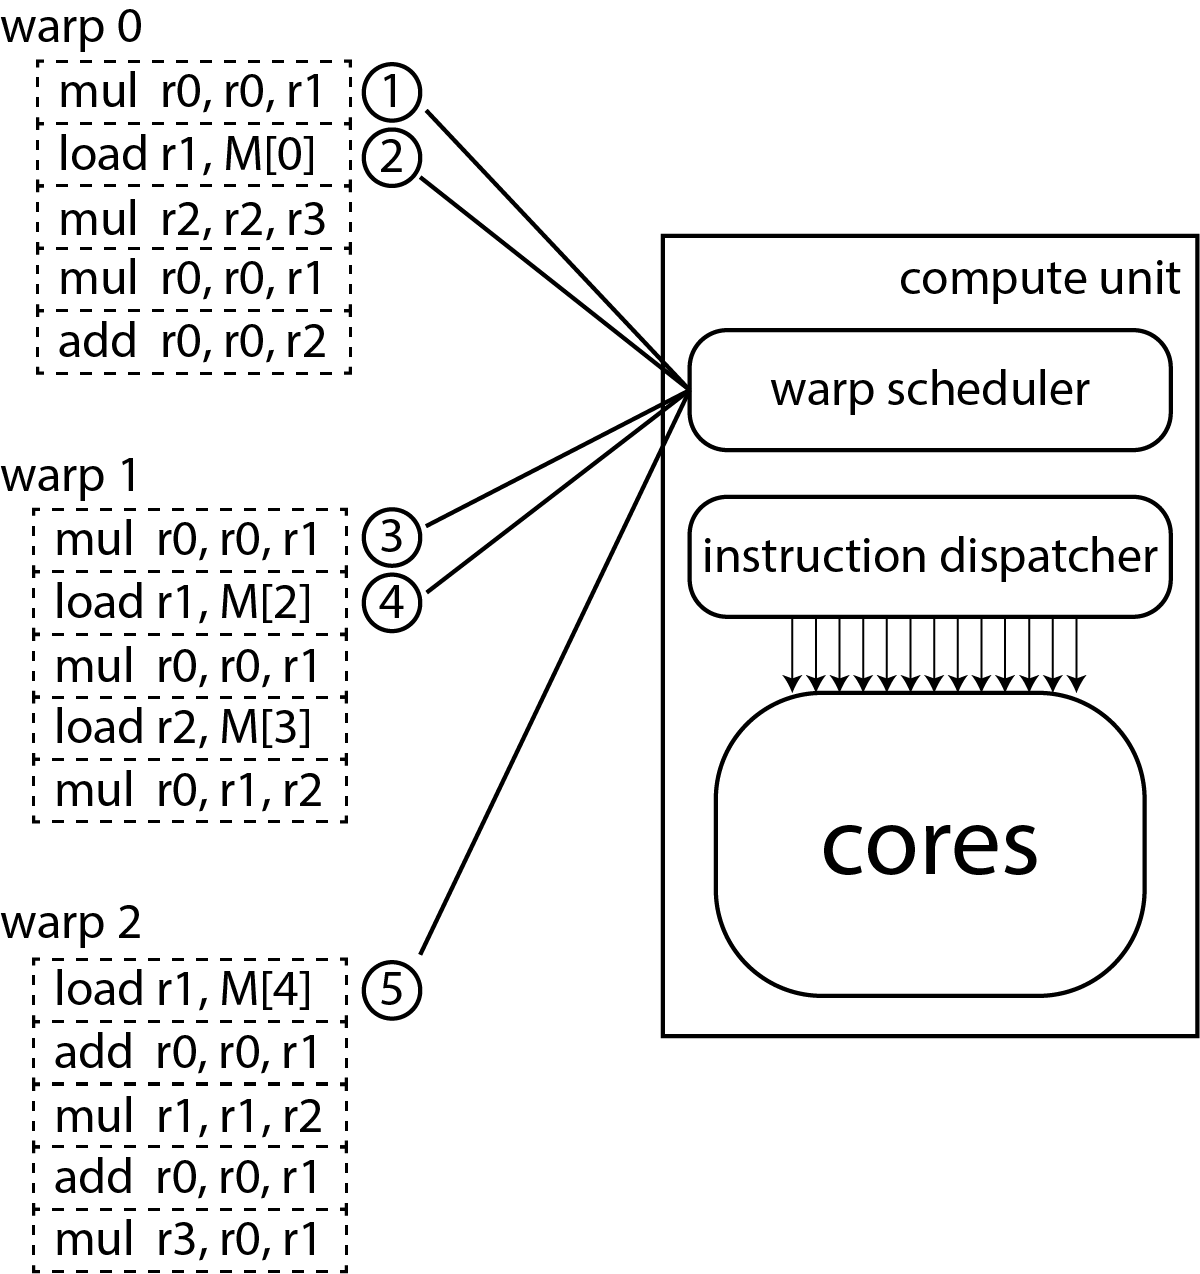
\includegraphics[width=0.45\linewidth]{TLP.png}

\caption{Illustration of the thread-level parallelism: the warp scheduler first issues instructions (1) and (2) of warp 0 and be blocked by (2), as it is long-latency global memory access instruction. Instead of waiting for the finish of this instruction, the warp scheduler fetches instructions from the warp 1 to keep the GPU busy. \label{tlp_fig}}

\end{figure}


Without enough thread-level parallelism, the single-image CNNs inference needs to seek latency hiding from the other mechanism: instruction-level parallelism. Instruction-level parallelism hides the latency in a single thread by issuing independent instruction simultaneously. If an instruction is independent with its previous instructions, this instruction can be issued no matter whether the previous instructions have finished or not. As shown in Figure \ref{ilp_fig}(b), the first four instructions load four independent values from global memory, which are independent of each other. The second instruction can be issued even if the first instruction has not finished. It usually relies on compilers to use instruction scheduling and register reallocation to reorder the instructions to maximize the instruction-level parallelism. The code in Figure \ref{ilp_fig}(a) does the same work with Figure \ref{ilp_fig}(b) without any instruction-level parallelism. Every addition instruction needs the value loaded by its previous instruction, and every global memory access instruction needs to wait its previous addition instruction to free the register (\texttt{r1}).

\begin{figure}[h!]
\centering

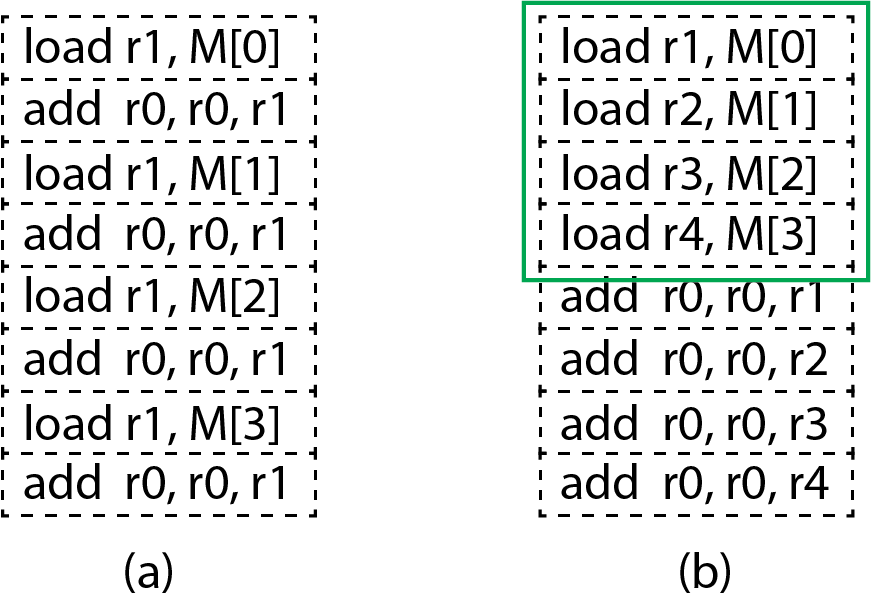
\includegraphics[width=0.45\linewidth]{ilp.png}

\caption{Illustration of the instruction-level parallelism \label{ilp_fig}}

\end{figure}


% Therefore, great care should be taken to manage the dependency among operations for single-image convolution neural network inference.

% The instruction-level parallelism is to issue long latency independent instruction pipelinely. The compilers are responsible relies on independent operations that can be issued independently. The ILP relies on instruction scheduling to rearrange the instruction for higher ILP. It usually fusion the memory operands and arithmetic operands to hide the latency. For example, consider the Code 100 which accumulates four floating-point number in memory and a virtual GPU with memory latency be 2 cycles, and floating-point addition takes 1 cycle. The ratio is chosen to simplify the illustration, and the ratio is usually much higher in real GPUs. Meanwhile, we insert nop if the value needed by the next instruction is not avaliable at that time, even though the global memory read is usually asynchronized and waited by a specific instruction. 


% The most trivial assembly code without instruction scheduling is shown in CODE 2. The global memory load issued at tick 2 is not available at tick 3. As the next instruction needs the value, a NOP instruction is inserted at tick 3 to guarantee the floating-point number addition instruction reads the correct value from the register \texttt{r2}. There is no instruction-level parallelism to hide the latency, and the total execution time is 13 cycles.


% On the other hand, the optimal assembly code is shown in CODE 3. At tick 3, instead of inserting a NOP instruction, the global memory load instruction of m1 is brought to this tick to keep the GPU busy. As the loading of \texttt{m1} does not depend on the result of the global memory load of \texttt{m0}, these two instructions can be issued independently. With instruction-level parallelism,  the total execution time is reduced to 9 cycles, and the GPU utilization is $100\%$. However, the \texttt{m1} should be loaded into another register (\texttt{r3}), as the value of \texttt{r2} will be used by following instructions. 


% on the other hand, the optimal assembly code is shown in CODE 3. The load operand of m1 is brought to tick 3 and the result is stored in another register. As the load of m1 does not dependent on the result of tick 2, it can be issued at tick 3. With ILP, the total execution time is reduced to 9 cycles. The instruction scheduling reduces the dependency among nearby instruction to improve the ILP.



However, two common constraints restrict the usage of instruction scheduling to improve instruction-level parallelism. The first constraint is introduced by memory barriers. It is a common optimization strategy to reduce the global memory access by letting threads of a workgroup copy data from global memory to the shared memory collaboratively when each value is used by multiple threads. As a thread needs the values loaded by others, before reading the shared memory, a memory barrier is needed to guarantee every value has been written into the shared memory. The compiler cannot schedule memory instructions across memory barriers, which restricts the instructions reordering and therefore the instruction-level parallelism.

Another constraint is the additional usage of registers. As shown in Figure \ref{ilp_fig}, the (a) only uses two registers, while the (b) needs five registers. The simultaneously loaded values need to be stored in different registers, which increases the registers usage significantly. As most GPUs do not support inter-threads register reuse, the registers need to be allocated to a warp during launching and reserved in the whole lifetime of the warp. If a memory-then-compute group, for example the first two instructions of Figure \ref{ilp_fig}(a), needs a great number of registers, pipelining too many such groups makes the registers become the bottleneck of the resource demands. It may reduce the number of warps that a compute-unit can hold and therefore decreases the thread-level parallelism, which is the primary mechanism for GPUs to hide the latency. As the number of warps is unknown during compilation time, the compiler cannot estimate the thread-level parallelism and may restrict the register usage to balance the thread-level parallelism and instruction-level parallelism. Therefore, the register usage also restricts the instruction-level parallelism. 


% However, instruction scheduling is not come for free, and there are mainly two constraints. The first constraint is introduced by memory barriers. There is a common optimization method for GPU kernel that all threads in a workgroup load data from the global memory to the shared memory collaboratively. As the thread needs to use the data loaded by other threads, before reading the shared memory, a shared memory barrier is needed to guarantee every value has been written into the shared memory. The compiler cannot schedule instructions across memory barriers, which limits the feasibility of instructions rearrangement and the instruction-level parallelism. Even if the GPU kernel code is rearranged manually, the pipeline is still not possible. In OpenCL, the shared memory barriers are applied to all shared memory of the workgroup. Therefore, even if we know that a group of arithmetic instructions only depends on one of the shared memory (denoted as S1) and another group of arithmetic instructions depends on another shared memory (denoted as S2), this relation cannot be expressed by high-level GPU programming languages. In the expression of OpenCL, the latter group of arithmetic instructions depends on both S1 and S2. On GPUs that guarantee the order of the shared memory operations, it is possible to load values from the global memory into the shared memory parallelly with assembly code. However, it is incredibly costly to write and optimize the assembly codes for every convolution setting.




% Another constraint is the additional usage of registers. As the value loaded from the global memory needs to be stored at different registers, pipelining the memory loading will significantly increase the number of registers used by a thread. As GPUs usually do not support dynamic register allocation, all used registers need to be reserved in the lifetime of the threads. More registers usage means fewer warps can be assigned for each compute-unit, which may reduce the thread-level parallelism. However, as discussed above, each compute-unit only has few warps for single-image inference, and the register usage is not a critical problem in this case. 




% To know more about latency hiding on GPUs, Volkov provided several high-quality materials \cite{volkov2010better, volkov2016understanding}.




\subsection{Memory Bandwidth and Energy Consumption of Embedded GPUs}
Another challenge of executing inference on embedded GPUs comes from hardware limitations. Most embedded GPUs and integrated GPUs use LPDDR4 or DDR4 as off-chip global memory, whose bandwidth is far less than GDDR6 and HBM2. The memory bandwidth of dual-channel LPDDR4 is about 30GB/s, while the bandwidth of GDDR6 and HBM2 is about 600GB/s and 1TB/s, respectively. Even worse, the limited memory bandwidth of mobile GPUs is shared by CPUs and other processors of the SoC, leading to even lower real memory bandwidth. It is much more easily for the global memory access to become the bottleneck on mobile GPUs. 

Additionally, the off-chip memory access consumes tens of times the energy compared with on-chip cache access and hundreds of times the energy compared with floating-point arithmetic. Even though energy consumption becomes to draw attentions of deep learning areas, it is still the last consideration when designing GPUs convolution algorithms, especially for GPUs that are powered by mains electricity. However, edge computing platforms are usually battery-powered. The energy consumption determines the battery lifetime. On embedded GPUs, it should be more careful when trading-off between global memory access and other operations.

% Additionally, the off-chip memory access consumes tens of times energy compared with on-chip cache access and hundreds of times the energy compared with floating-point addition and multiply. Even though energy consumption becomes to draw attention in the deep learning areas, it is the last consideration when designing convolution algorithms for GPUs that are powered by mains electricity. However, edge computing platforms are usually battery-powered. The energy consumption determines the battery lifetime.

% Therefore, when trading off between global memory access with other operations, global memory access is more undesirable on mobile GPUs than dedicated GPUs.



\subsection{Engineering Choice of Inference}

Last but not least, the engineering choice of the convolution algorithms for CNNs inference is usually different from that of CNNs training. For CNNs training, various neural network architectures and combinations of convolution parameters are examined to find the one with the best performance. In such a scenario, an algorithm that provides stable and acceptable performance for any convolution setting is preferred. It frees the practitioners from tuning the GPU kernels for every convolution parameter, and the practitioners can focus on the performance of the CNNs. However, for the CNNS inference, the neural network architecture and convolution parameter is fixed. In this stage, the goal becomes to optimize the GPUs convolution kernel codes for short inference time and low energy consumption. It is worth to adopt the convolution algorithm that achieves the fastest speed even if great efforts need to be paid for tuning.

% Last but not least, the engineering choice of inference is usually different from training. For deep neural network training, various convolution neural network architecture and combination of convolution setting are examined. In such a scenario, an algorithm that provides stable and acceptable performance for any convolution setting is preferred. It frees neural network developers from tuning the GPU kernels for every convolution setting. Thus neural network developers can focus on the performance of the neural networks. However, for inference, the architecture and settings of convolution neural network are fixed. Therefore, the goals become to optimize for short inference time and low energy consumption. It is worth to adopt the convolution algorithm that achieves the fast speed even if gert efforts need to be pard for tuning.




\section{Existing GPU Convolution Algorithms}

This section reviews several popular GPU convolution algorithms, which are unrolling-based convolution algorithms(\texttt{im2col} and \texttt{libdnn}), Winograd convolution algorithm, and direct convolution algorithm. The FFT-based convolution algorithm is not discussed. It performs well only with large convolution filters, while the state-of-the-art CNNs mainly use small convolution filters.


\subsection{Unrolling-based Convolution Algorithms}

Unrolling-based convolution algorithm is the most popular GPU convolution algorithm for CNNs training. The key idea is to transform the sliding-window convolution, which is hard to optimize, into well-studied matrix multiplication \cite{im2col}. As shown in Figure \ref{im2col}, each convolution filter is flattened into a row, while the input images are unrolled into columns of a matrix. Each pixel of the output image is then computed by dot-product of each column of the unrolled input matrix with the corresponding convolution filter row. The transformation is named \texttt{im2col}, and we denoted this unrolling-based convolution algorithm as \texttt{im2col} convolution. It allows performing convolution with heavily optimized GEMM libraries, such as clBLAS and cuBLAS.

\begin{figure}[h!]
\centering

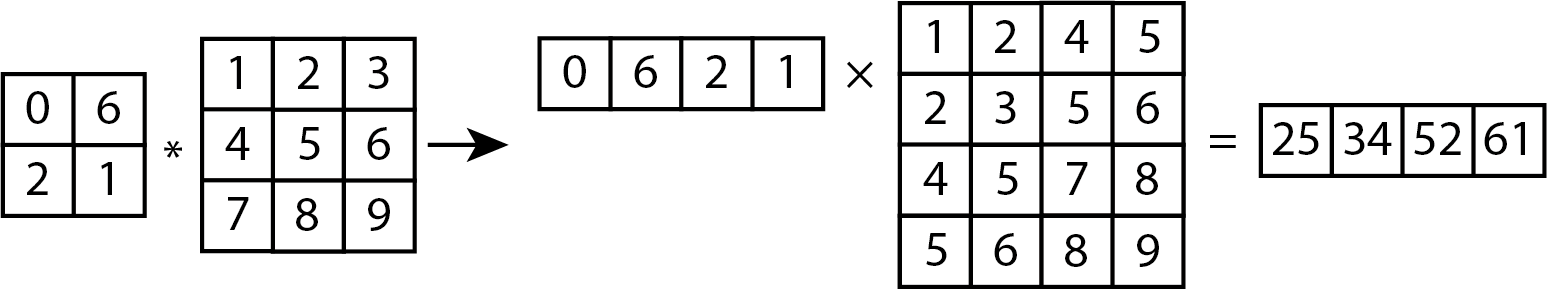
\includegraphics[width=0.8\linewidth]{im2col.png}

\caption{Illustration of the \texttt{im2col} convolution algorithm \label{im2col}}

\end{figure}

The limitations of the \texttt{im2col} convolution are that it wastes memory to store duplicated input images and introduces significant global memory access overhead. As the BLAS libraries provide GEMM as a standalone function, \texttt{im2col} convolution separates the \texttt{im2col} and matrix multiplication to two GPU kernels. The \texttt{im2col} GPU kernel needs to store the unrolled input matrix into global memory, and then the GEMM kernel needs to load the unrolled input matrix back from global memory. As the size of the unrolled input matrix is \texttt{kernel\_size} times of the input images, it incurs significant global memory bandwidth overhead, especially for embedded GPUs.

Another unrolling-based convolution implementation named \texttt{libdnn} \cite{tschopp2016efficient, Tschoppgithub} eliminates the global memory bandwidth overhead by combining the \texttt{im2col} and GEMM into a single GPU kernel. When performing the tiled matrix multiplication, each tile of the unrolled input matrix is constructed on the fly only by the workgroups that need this tile. As all tiles of the unrolled input matrix are only stored in on-chip memory and discarded after matrix multiplication, they do not need to be written to and read from the global memory.

%As illustrated in Figure 100, w

Even though \texttt{libdnn} eliminates the storage and bandwidth overhead incurred by the unrolled input matrix, the performance of \texttt{libdnn} convolution is not always better than the \texttt{im2col} convolution, especially for CNNs training. First, as the \texttt{im2col} kernel only performs index calculation and global memory copy, which can be heavily pipelined with thread-level parallelism, considering the state-of-the-art dedicated GPUs have up to 1TB/s global memory bandwidth. Also, as each tile of the unrolled input matrix is used by multiple workgroups, many workgroups need to unroll the same tile. The unrolling operation involves complex index calculation and irregular global memory access, which are unfriendly to GPUs.


% Unrolling-based convolution is the most popular GPU convolution algorithm. The key idea is to convert the sliding-window convolution, which is hard to optimize, into well-studied matrix multiplication. The local regions of input images are repeated and unrolled into columns of a matrix, and the convolution kernels are unrolled into rows of another matrix. The unrolling procedure of the input images is named \textit{im2col}. Each pixel of the output image is the dot product of the corresponding column of the input matrix and row of the kernel matrix. Thus the whole output images are the product of the input matrix and the kernel matrix, and there are many efficient and highly-optimized libraries for matrix multiplication(GEMM), such as cuBLAS and clBLAS. I found a great blog about this progress \cite{im2col}.


% As the BLAS libraries provide GEMM as a standalone function, most implementation of the unrolling-based convolution separates the \textit{im2col} and matrix multiplication into two GPU kernels. The \textit{im2col} kernel first loads input images from global memory and writes the unrolled input matrix back to global memory, and the unrolled input matrix is then loaded from global memory by GEMM. The size of the unrolled input matrix is \texttt{kernel\_size} times of the input images, which incurs significant global memory bandwidth overhead for edge computing platform due to the unnecessary global memory read and write.

% Another unrolling-based convolution implementation named \textit{libdnn} eliminates the global memory bandwidth overhead by combining the \textit{im2col} and GEMM into a single GPU kernel. Instead of reading the unrolled input matrix, each workgroup of \textit{libdnn} loads original input images and unrolls it into a tile of the unrolled input matrix that processed by this workgroup just-in-time. The tile of the unrolled input block is multiplied with the corresponding tile of the kernel matrix and then discarded after usage. As the unrolled input matrix is constructed and used by the same kernel, it does not need to be stored in, read from, and written back to the global memory. The code is available at \cite{Tschoppgithub} and there is also a technical report \cite{tschopp2016efficient}. 

% It should be noticed that even though \textit{libdnn} eliminates the storage and bandwidth overhead incurred by the unrolled input matrix, the performance of \textit{libdnn} is not always better, especially for convolution neural network training. First, the state-of-the-art dedicated GPUs have up to 1 TB/s global memory bandwidth. Together with the thread-level parallelism, the read and write of the unrolled input matrix only cost negligible time compared with the matrix multiplication. Also, as each tile of the unrolled input matrix is used by different workgroups, many workgroups need to unroll the same tile. The unrolling operation involves complex index calculation and irregular global memory access, which are unfriendly to GPUs.


\subsection{Winograd Convolution Algorithm}

Winograd convolution algorithm was documented in 1980, but it has not been widely used by CNNs until 2015 \cite{lavin2016fast}. The Winograd convolution algorithm first divides the output images into tiles and computes each tile as follows, $$A^{T}[(Gg) \odot (B^{T}d)]$$ where $g$ is the convolution filters, $d$ is the input images. The $A$, $B$, and $G$ are transformation matrices, which are constants for a given value of tile size and convolution filter size. For Winograd convolution with tile size $M$ and convolution filter size $R$, each tile needs $(M+R-1)^{2} \times R^{2}$ times multiplication, while the unrolling-based convolution and direct convolution need $M^{2}R^{2}$ times multiplication. Meanwhile, the Winograd convolution also increases the thread-level parallelism, as the matrix multiplication of smaller transformed matrices has more independent workload and therefore more warps.

The reduction of the number of multiplication is at the cost of extra global memory access and floating-point addition. As the convolution filters are also constants for CNNs inference, only the transformation of input images and inverse transformation of the output images need to be performed. The number of global memory access and addition increases quadratically with the tile size and convolution filter size, or formally, $$A(transformation\_cost) \in \mathcal{O}(M^{2} + R^{2})$$ For large convolution filters, the memory access and addition complexity of the transformation may overwhelm the benefits of multiplication reduction for large convolution filters. Also, the transformations introduce substantial global memory access, which is expensive for embedded GPUs due to the bandwidth limitation and energy consumption. 

% The Winograd convolution algorithm \cite{lavin2016fast} was proposed in 1980, but it has not been widely used by convolution neural network until 2015. It divides the input images into small tiles and transforms both the tiled input images and convolution kernels into a group of small matrices. Each matrix of the transformed input matrices group is multiplied with the corresponding matrix of the transformed kernel matrices group. As the size of the transformed matrices is much smaller than the original matrices, the total arithmetic numbers are reduced. For example, if the kernel size is $R \times R$ and the tile size is $M \times M$, the standard algorithm uses $M^{2}R^{2}$ multiplications while the Winograd convolution only needs $(M+R-1)^{2} \times R^{2}$ multiplications for each tile.

% However, the number of addition and constant multiplications required by the Winograd transforms increases quadratically with the kernel size. Thus for large convolution kernels, the memory access and the arithmetic complexity of the transformation will overwhelm the benefits of multiplication reduction. Also, the transforms introduce substantial global memory access, while global memory is expensive on mobile GPUs due to the bandwidth limitation and energy consumption.


\subsection{Direct Convolution Algorithm}

Direct convolution is the convolution algorithm that follows the definition of convolution \cite{krizhevsky2012cuda}. The convolution filters slide over the input images, and the dot-product between their elements are computed and accumulated into the corresponding output images. Many studies \cite{perrot2016optimized, iandola2013communication, chen2017optimizing, li2015fast} optimized global memory access and data reusing in on-chip memory to speedup the trivial direction convolution algorithm. These optimizations are similar to that of matrix multiplication, which mainly consists of collaboratively loading the data from global memory and assigning more work to a thread to reuse the register. Generally, the direct convolution needs less shared memory compared with other convolution algorithms, as it caches the input images rather than the transformed or unrolled data. Meanwhile, the direct convolution algorithm usually has no complex index and memory offset calculation and therefore needs fewer arithmetic instructions.



% Direct convolution is the convolution algorithm that follows the definition of convolution \cite{krizhevsky2012cuda}. The convolution kernels slide along the input images, and the dot product between the convolution kernel and the slid image region is accumulated to the corresponding output image. From the aspect of memory shared usage, the direct convolution needs the least shared memory as it caches the input image rather than the unrolled input matrix. Meanwhile, as direct convolution does not need to do the complex index and memory address calculation, the scalar arithmetic operands of direct convolution are much less than the unrolled-based convolution.


\begin{algorithm}
\caption{Direct Convolution Algorithm \label{dcap}}
\begin{algorithmic}[1]

\Function{conv\_cache\_filter}{}%{$img\_global$, $filter\_global$, $out\_global$}

    \For{$1$ to IN\_CHANNELS}
        \State \Call{load}{$img\_global$, $img\_shared$}
        \For{$1$ to OUT\_CHANNELS\_PRE\_THREAD}
            \State \Call{load}{$filter\_global$, $filter\_shared$}
            % \State Load convolution filters into shared memory
            \State \Call{barrier}{LOCAL\_MEM}
            \State add $filter\_shared \bigodot img\_shared$ into $out\_reg$
        \EndFor 
    \EndFor
    \State \Call{save}{$out\_reg$, $output\_global$}
\EndFunction
\State
\Function{conv\_nocache\_filter}{}%{$img\_global$, $filter\_global$, $out\_global$}

    \For{$1$ to IN\_CHANNELS}
        \State \Call{load}{$img\_global$, $img\_shared$}
        \State \Call{barrier}{LOCAL\_MEM}
        \For{$1$ to OUT\_CHANNELS\_PRE\_THREAD}
            % \State \Call{load}{$filter\_global$, $filter\_shared$}
            % \State Load convolution filters into shared memory
            
            \State add $filter\_global \bigodot img\_shared$ into $out\_reg$
        \EndFor
    \EndFor
    \State \Call{save}{$out\_reg$, $output\_global$}
\EndFunction

\end{algorithmic}
\end{algorithm}

% However, direct convolution usually needs great efforts to tune the GPU kernels to get a reasonable speed, let alone the optimal speed. compared with the \textit{libdnn}, whose critical hyperparameters are only the size of the workgroup and workload of each workgroup, direct convolution has all these hyperparameters in addition with much more other hyperparameters. For example, the number of the output channels dealt by each workgroup affects how many times the input images are read and the number of the warps. Meanwhile, whether the filter should be loaded collectively and cached in the shared memory is always a hard choice, especially for single-image inference, whose latency cannot be hidden by TLP. If not, then each thread needs to use kernel size times global memory load operands, and all threads within a workgroup load the same data at the same time. The most serious problem is that the compiler may try to pipeline the kernel loading as it is global memory operands. A great number of registers are needed, which is not necessary if convolution kernels are stored in the shared memory. Also, even with the L2 cache, the overhead caused by issuing the global memory still quite substantial. On the other hand, if the filter is loaded collectively, as shown in Algorithm \ref{dcap}, then a shared memory fence needs to be put after every convolution kernel load. The instructions between such two fence are all arithmetic instructions, so the compiler cannot fusion the memory instructions and arithmetic instruction to hide the latency, which significantly hurts the ILP.

However, there are lots of parameters and decisions that affect the performance of the direct convolution, and it usually needs more efforts to tune the direct convolution GPU kernels to find out the optimal combination of parameters. The main computation of unrolling-based convolution and Winograd convolution is matrix multiplication, whose key parameters are only the tile shape and workload per threads. Direct convolution algorithm has all GEMM's parameters and additional parameters that are difficult to choose, such as the output channels processed per threads and whether the convolution filters and outputs should be cached in the shared memory.

Among all implementation choices of direct convolution kernels, the most critical contradiction for single-image CNNs inference is that whether to cache the convolution filters in the shared memory or not. The pseudocode of the caching implementation is shown in Algorithm \ref{dcap} (\texttt{CONV\_CACHE\_FILTER}), where the convolution filters are loaded from global memory and cached in the shared memory collaboratively. Each thread only needs to load a small portion of rather than the whole convolution filters from the global memory, which reduce the global memory bandwidth pressure. However, a memory barrier needs to be put before performing the dot-product to guarantee all weights of the convolution filters have been written into the shared memory. For CNNs training, the latency is hidden by thread-level parallelism, while for CNNs inference, the instruction-level parallelism is the primary mechanism for latency hiding. There are only \texttt{filter\_size} times arithmetic and no memory loading between any two adjacent inner barriers (Line 6). It limits the instructions scheduling significantly, as the compiler cannot move memory instructions across memory barriers. Even worse, as the convolution filters are stored in the same piece of the shared memory, the global memory loading instructions cannot be issued until the previous arithmetic has finished. It entirely prevents the compiler from fusing the memory instructions and arithmetic instructions to hide the latency.



On the other hand, the pseudocode of the non-caching implementation is listed in Algorithm \ref{dcap} (\texttt{CONV\_NOCACHE\_FILTER}). In this case, the dot-product involves filter size times global memory access and \texttt{filter\_size} times arithmetic. There are \texttt{output\_channel\_per\_thread $\times$ filter\_size} times independent arithmetic and memory instructions between two adjacent memory barriers for the compiler to reorder to hide the latency. However, there is a noticeable drawback if the convolution filters are not loaded collaboratively. As each thread needs to load all convolution filters, the non-caching implementation needs much more global memory access. The L2 cache may ease the problem, but the overhead is still substantial. The duplicated global memory access also increases the registers used to store the same values. To load the convolution filters simultaneously, the loaded values need to be stored in different registers. Pipelining the calculation within a dot-product needs \texttt{filter\_size} times registers, which significantly increases the register usage and therefore restricts the instruction-level parallelism. Meanwhile, as the latency of memory instructions are usually longer than that of floating-point arithmetic instructions, the ratio of these two kinds of instructions of direct convolution is unfriendly to instruction-level parallelism.

% Usually, for neural network training, which has enough TLP, caching the filter will benefit. On the other hand, for single-image neural network inference, which mainly relies on ILP as discussed above, not caching the filter is better.



% \begin{algorithm}
% \caption{Direct Convolution Algorithm \label{dcap}}
% \begin{algorithmic}[1]

% \Function{convolution}{input, filter, output}
    
%     \State \_\_local float in\_img\_cache[TILE\_WIDTH][TILE\_WIDTH]
%     \State \_\_private float out\_img\_cache[OUTPUT\_CHANNELS] = {.0}


%     \For{$in\_channel \gets 1$ to input\_channels}
%         \State
        
%         \State in\_cache[local\_id.y][local\_id.x] = input[in\_channel][global\_id.y][global\_id.x]
%         \State \Call{barrier}{LOCAL\_MEM}
%         \State
        
%         \For{$out\_channel \gets 1$ to OUTPUT\_CHANNELS}
%             \State
        
%             \State filter\_cache[local\_id] = filter[in\_channel][out\_channel][local\_id]
%             \State \Call{barrier}{LOCAL\_MEM}
%             \State
    
%             \For{$r \gets 1$ to FILTER\_WIDTH}
%                 \For{$c \gets 1$ to FILTER\_WIDTH}
%                     \State out\_reg[$out\_channel$] += in\_cache[local\_id.y+r][local\_id.x+c] * filter\_cache[r*FILTER\_WIDTH+c]
%                 \EndFor
%             \EndFor
%         \EndFor
%         \State
        
%     \EndFor
%     \State
    
    
%     \For{$out\_channel \gets 1$ to OUTPUT\_CHANNELS}
%         \State output[bucket\_id][global\_id.y][global\_id.x] = out\_reg[bucket\_id]
%     \EndFor

% \EndFunction

% \end{algorithmic}
% \end{algorithm}


\section{Methodology} %: Asocial Convolution Algorithm


In this paper, we proposed a GPU convolution algorithm for single-image CNNs inference on embedded GPUs, named Instruction-Level Parallelism Maximizing convolution (ILP-M convolution). It is based on the direct convolution algorithm but optimized for single-image by eliminating the memory barriers without introducing duplicated convolution filters loading. The key idea is to map threads to output channels and iterate along pixel, instead of mapping threads to pixels and iterate along output channels, as illustrated in Algorithm \ref{ILP-M}. Some secondary well-known optimization strategy, such as transposing the output images for coalescing write, are ignored for simplification.

% In this report, we proposed a convolution algorithm specialized for single-image convolution neural network inference on mobile GPUs, named HNTMP convolution\footnote{The code is available at: https://github.com/jizhuoran/sj\_convolution}. It is based on the direct convolution algorithm but eliminates the tradeoff between caching the filter or not. The key idea is to map threads to output channels and iterate along pixel, instead of mapping threads to pixels and iterate along output channels. The rough idea is shown in Algorithm \ref{hmtp}.



For ILP-M convolution, all threads in the same workgroup also copy input images from the global memory into the shared memory collaboratively, and therefore a memory barrier is needed before accessing the input images in the shared memory. In this stage, each thread is mapped to a pixel. After that, threads of a workgroup are mapped to output channels rather than pixels. Each thread calculates the whole output image tile of its corresponding output channel, while for direct convolution, each thread calculates its corresponding pixel of all output channels. As all pixels of the same output channel is calculated with the same convolution filter, each thread loads and only needs to load one convolution filter (\texttt{filter\_size} values) for \texttt{workgroup\_size} arithmetic. Figure \ref{ccoc} illustrates the difference of convolution filters footprint between ILP-M convolution and direct convolution. The ratio of arithmetic instructions to global memory instructions is \texttt{workgroup\_size}, providing substantial space for compiles to reorder the instructions to hide the latency.

ILP-M convolution algorithm further reduces the register usage by iterating the weights of the convolution filter in the outer loop. Each time, the thread only needs to load one weight of the convolution filter, multiples it with all pixels of the input image tile and accumulates the result into the output image tile. After calculating the dot-product between all input channels and their corresponding convolution filters, the output images tile is written back to the global memory. As the threads compute a tile of the output images of different output channels, this global memory write is not coalesced due to the data layout of the output images. ILP-M convolution allows to chose whether to use shared memory to transpose the output images tiles and therefore, the output images tiles can be coalesced written back to global memory.

% To further reduce the registers used for storing the convolution filter, a thread will load one weight of the filter corresponding to its assigned output channels each time. This weight is multiplied with the whole input image tile, and the products are accumulated into the output image tile. 

% Same with the original direct convolution algorithm, all threads of a workgroup first load the input image tile from the global memory into the shared memory collaboratively. In this stage, each thread is mapped to a pixel. After that, each thread is mapped to an output channel and computes the whole output image tile of this output channel. As all pixels of an output channel is calculated with the same convolution filter, each thread loads and only needs to load one convolution filter in its whole lifetime. In contrast, for the original direct convolution algorithm, each thread needs to load \texttt{workgroup\_size} convolution filters to compute the same number of output channels. The difference is illustrated in Figure \ref{ccoc}.


\begin{figure}[h!]
\centering
\captionsetup[subfloat]{farskip=2pt,captionskip=1pt}


\subfloat[Direct Convolution]{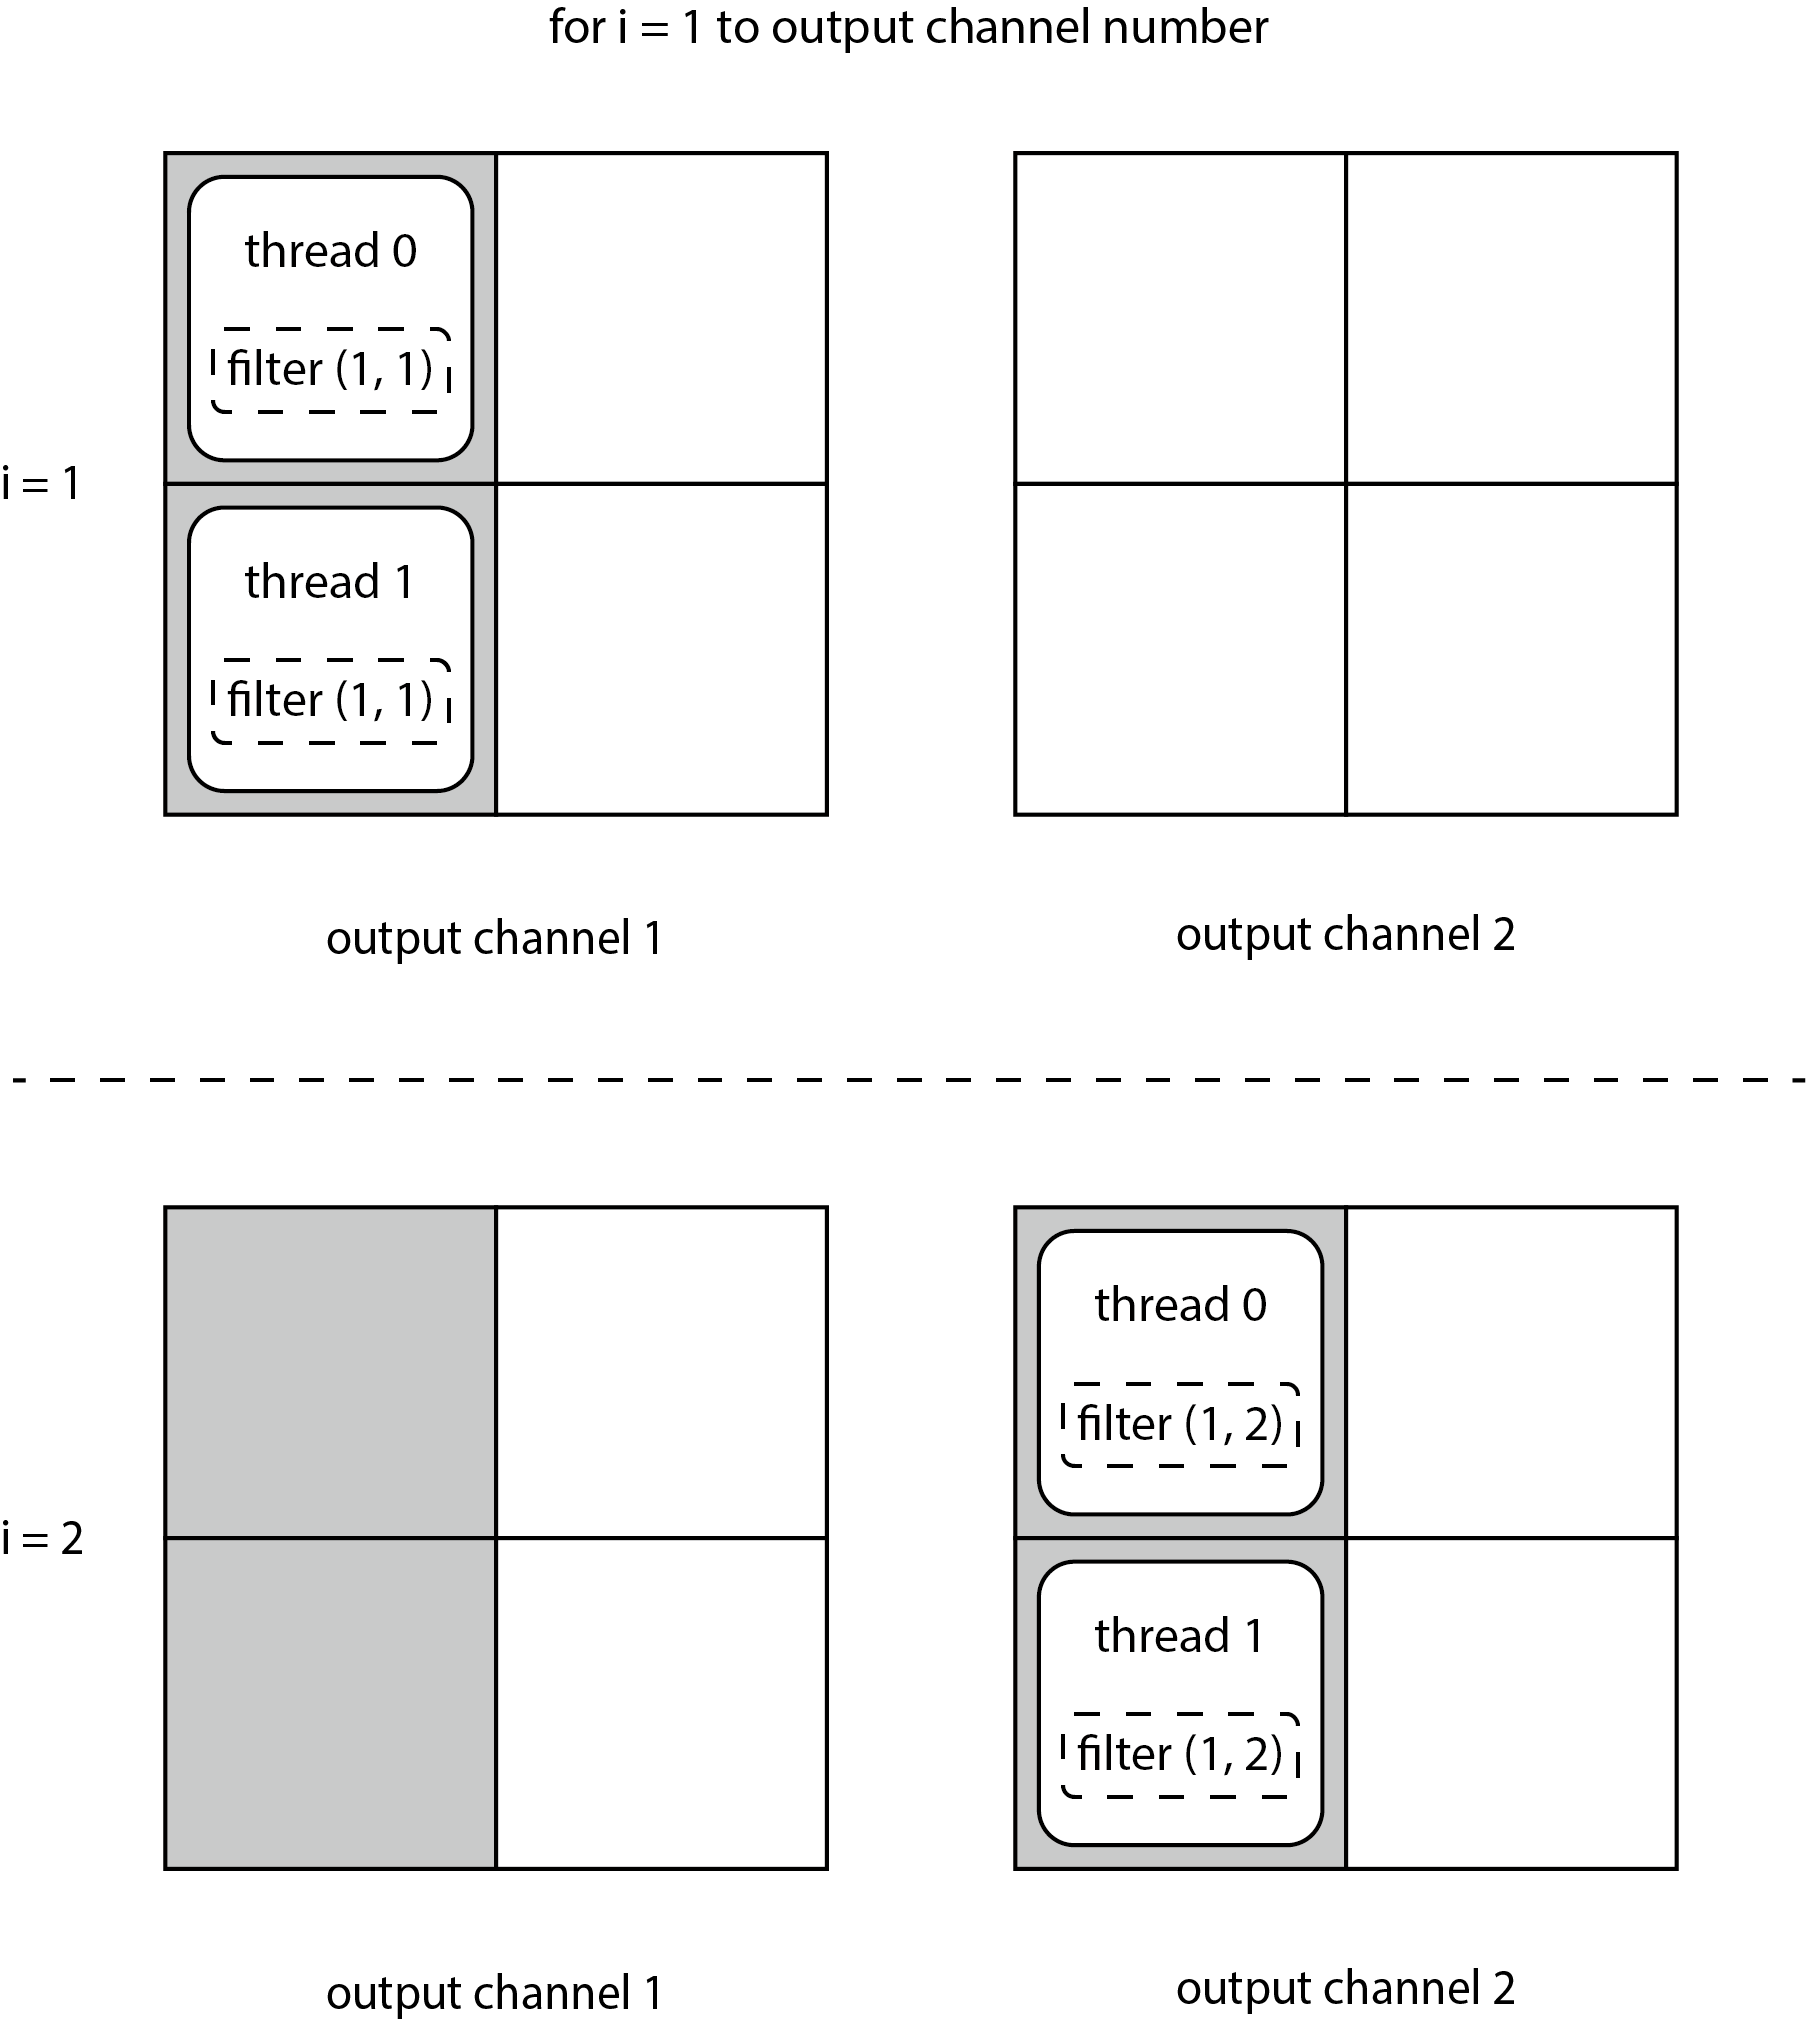
\includegraphics[width=0.45\linewidth]{cc.png}}
\hspace{1.2cm}
\subfloat[ILP-M Convolution]{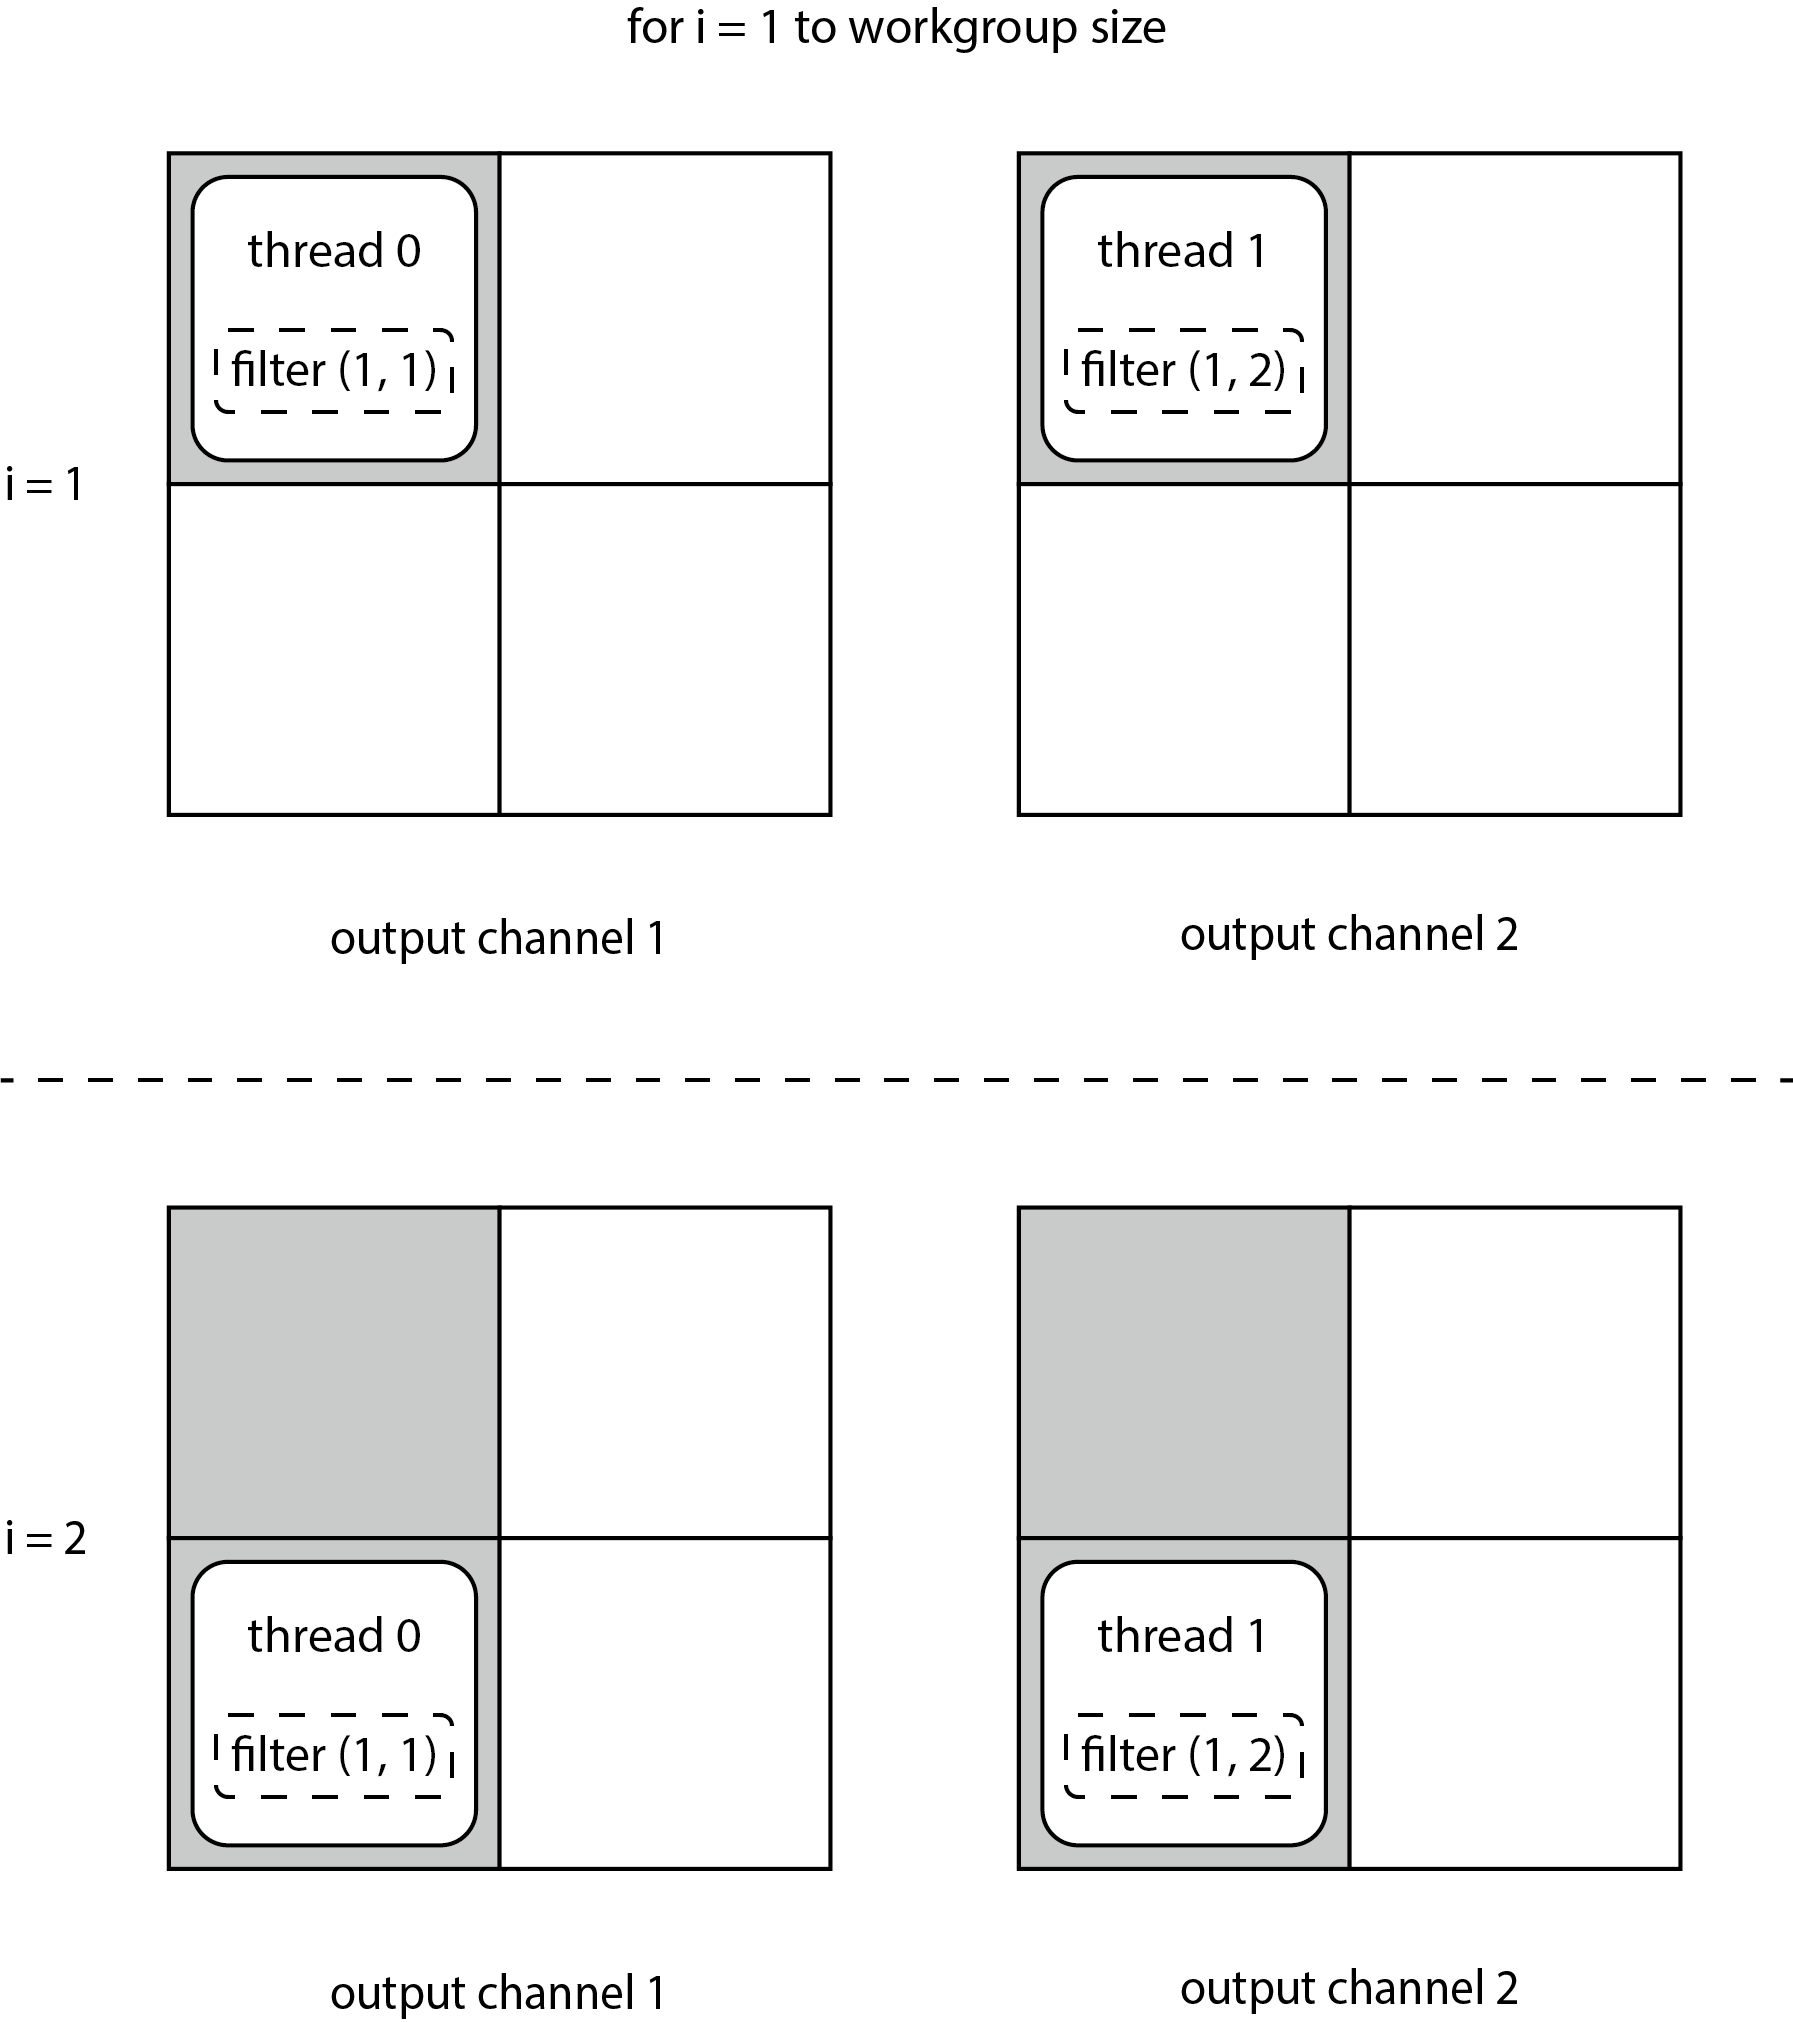
\includegraphics[width=0.45\linewidth]{oc.png}}

\caption{Difference of Direct Convolution and ILP-M Convolution. $filter(i, j)$ refers to the convolution filter of input channel $i$ and output channel $j$. The gray square indicates this pixel has been calculated. \label{ccoc}}

\end{figure}






% We proposed an improved version the direct convolution algorithm based on the characteristic of the single-image convolution neural network inference on edge computing platforms. The key idea of our method is to map threads of a workgroup to different output channels and let each threads compute all pixels within the sub-region of its assigned output channels. The algorithm is shown in Algorithm 100. 

% It should be noticed this pseudocode only used to illustrated the idea, it ignores the boundary check and assume the output image is smaller enough to fit in one workgroup. Meanwhile, it ignored many optimization mechanism, such as reorganized the kernel matrix for coalescing read. The very detailed algorithm is shown in the appendix.


% Our method first maps threads to the pixels of the input images to collaboratively load the input images into the shared memory, which is same with the original direct convolution algorithm. After that, instead of let each thread to compute one pixel of several output channels, our methods map each thread to one output channel and let it compute all pixels of this output channel.



\begin{algorithm}
\caption{ILP-M Convolution Algorithm \label{ILP-M}}
\begin{algorithmic}[1]

\Variables
 \State LOCAL\_DIM\_\#, the shape of the workgroup at dim\#
 \State C, R, S, K, the input channel, filter width, filter height, output channel
\EndVariables
\State
\Function{convolution}{input, filter, output}
    
    % \State 
    % \State \_\_local float in\_img\_cache[TILE\_SIZE\_Y][TILE\_SIZE\_X]
    % \State \_\_private float out\_img\_cache[DIM] = {.0}
    % \State 
    % \State offset\_x $\gets$ group\_id.x * LOCAL\_DIM\_X
    % \State offset\_y $\gets$ group\_id.y * LOCAL\_DIM\_Y
    % \State
    
    \For{$in\_channel \gets 1$ to input\_channels}
        
        \State 
        
        \State \Call{load}{$img\_global$, $img\_shared$}
        \State \Call{barrier}{LOCAL\_MEM}
        \State 
        
        % \For{$i \gets 1$ to $\lceil \frac{TILE\_SIZE}{LOCAL\_DIM} \rceil$}
        %     \State dest $\gets$ i * DIM + local\_id
        %     \State destY $\gets$ dest $/$ TILE\_SIZE\_X
        %     \State destX $\gets$ dest $\%$ TILE\_SIZE\_Y
        %     \State srcY $\gets$ offset\_y + destY - HALF\_FILTER\_WIDTH
        %     \State srcX $\gets$ offset\_x + destX - HALF\_FILTER\_WIDTH
        %     \State in\_img\_cache[destY][destX] = input[in\_channel][srcY][srcX] \Comment{ignore boundary check}
        %     % \State in\_cache[local\_id.y][local\_id.x] = input[in\_channel][global\_id.y][global\_id.x]
        % \EndFor
 
        \For{$r \gets 1$ to FILTER\_WIDTH}  
            \For{$s \gets 1$ to FILTER\_WIDTH}
                \State filter\_reg $\gets$ filter[i][r][s][local\_id] \Comment{the filter is reorganized by [C][R][S][K] for coalescing read}
                \For{$wy \gets 1$ to LOCAL\_DIM\_Y}  
                    \For{$wx \gets 1$ to LOCAL\_DIM\_X}
                        \State out\_reg[wy][wx] += filter\_reg * $img\_shared$[wy + r][wx + s]
                    \EndFor
                \EndFor
            \EndFor
        \EndFor
        \State
    
    \EndFor
    \State
    
    % \Comment{transpose the output images for coalescing write may improve the speed}
    \For{$wy \gets 1$ to LOCAL\_DIM\_Y}  
        \For{$wx \gets 1$ to LOCAL\_DIM\_X}
            \State save $out\_reg[wy][wx]$ to global memory
            % \State output[LOCAL\_DIM * global\_id.z + local\_id][offset\_y+wy][offset\_x+wx] = out\_reg[wy][wx]
        \EndFor
    \EndFor

\EndFunction


\end{algorithmic}
\end{algorithm}



ILP-M convolution algorithm inherits all advantages of direct convolution in terms of the shared memory usage and arithmetic operations. As it is designed for single-image CNNs inference, ILP-M convolution hides the latency mainly by instruction-level parallelism rather than thread-level parallelism. ILP-M convolution algorithm maximizes the instruction-level parallelism by eliminating the instruction dependency and reducing the register usage. Meanwhile, the ratio of arithmetic instructions to memory instructions is quite high, providing enough space for compilers to fuse these two kinds of instructions to hide the latency.


% HNMTP convolution inherits all advantages of direct convolution, which is regarded as the most suitable convolution algorithm for single-image convolution algorithm for mobile GPUs. Meanwhile, our convolution algorithm solves the dilemma of whether or not to cache the filter. HNMTP convolution uses the same number of global memory access and registers with the caching schema without introducing shared memory barrier for convolution filter loading. Compared with the caching schema, our convolution algorithm avoids shared memory barriers. There are \texttt{kernel\_size} global memory reads and \texttt{kernel\_size} times \texttt{workgroup\_size} floating-point arithmetic instruction between the shared memory barrier for input image tile. The compiler has enough instruction scheduling feasibility to fusion the global memory operands and arithmetic operands to hide the latency. Even only with few warps, the ILP keeps the GPU busy and therefore achieves high GPU utilization.

% On the other hand, different from the non-caching schema, HNMTP convolution does not introduce duplicated global memory instructions nor waste registers to store the same values. To pipeline N computing groups, HNMTP convolution only needs N register to store the filters, while the non-caching schema needs N times \texttt{kernel\_size} registers. In other words, for the same number of registers, N times computing groups can be pipelined to hide the latency compared with the non-caching schema. Also, even with L2 cache, which relieves the burden of global memory bandwidth, the duplicated global memory read instructions of the non-caching schema still incurs instruction issuing overhead and L2 cache access latency.

% It over-performs the common direct convolution method, as it solve the contradictions of whether the filter should be cached. As different threads need different filters, in other words, a thread do not need the filter value loaded by other threads, no sync is needed. Unlike the cache choice, which waste register to store and issuing global memory loading instructions for same filter values, our method loads and stores each filter only once.

% In our method, the threads read each filter only once the there is no need to sync as a thread does not use filters loaded bu other threads. Therefore, the compiler is free to rearrange the filter load and arithmetic operations to fusion the memory operands and arithmetic operands to hide the latency. Meanwhile, the threads of the same work-group do not waste register to store the same registers, therefore for same number of register, our method could pipeline more global memory loading to improve the ILP.




\section{Evaluation and Experiments}

We implemented ILP-M convolution kernels\footnote{The code is available at: https://github.com/jizhuoran/sj\_convolution} with OpenCL for portability to embedded GPUs and integrated GPUs. We also implemented an auto-tuning library to chose the optimal combination of the kernel parameters, such as the tile size and workload per thread. We compared the five GPUs convolution algorithms discussed in previous sections, which are \texttt{im2col} convolution, \texttt{libdnn} convolution, Winograd convolution, direct convolution, and our ILP-M convolution. Other convolution kernels are also written in OpenCL, and we used the GEMM function of clBLAS as the matrix multiplication kernels.

The experiments were conducted on three typical and distinctive platforms: mobile GPUs (Arm Mali-G76 MP10), integrated GPUs (AMD Radeon Vega 8), and high-end dedicated GPUs (AMD Radeon VII). The details of the model type and configuration are shown in Table \ref{platform}. The high-end dedicated GPUs usually have many compute-units and dedicated graphics memory with extremely high bandwidth. Integrated GPUs share host memory with CPUs, whose bandwidth is quite limited. The compute-units of integrated GPUs are usually the same as the dedicated GPUs, while the number of compute-units is usually less than the high-end dedicated GPUs. For embedded GPUs or mobile GPUs, the memory bandwidth is similar to the integrated GPUs, but the compute-unit is simple and has less arithmetic logic units. 



% We ran speed experiments with ResNet, which is the most popular and state-of-the-art convolution neural networks. The first convolution layer, whose convolution filter is $7\times7$, is ignored in our experiments. All no-1x1 convolution layers in Reset have $3\times3$ convolution filters except the first one. There are only three kinds of no-1x1 convolution layers of ResNet and the difference between different ResNet is only the number of these convolution layers, which is summarized in Table \ref{reset_setting}.


\begin{table*}[h]
\centering
\caption{Experiment Devices Configuration\label{platform}}
\begin{tabular}{l|l|l|l|l|l}
\hline
Model              & Global Memory Type  & Memory Bandwidth & CU & ALUs / CU & Total ALUs \\ \hline
AMD Radeon™ VII    & HBM2                & 1024 GB/s        & 60 & 64        & 3840       \\
AMD Radeon™ Vega 8 & DDR4 single-channel & 25 GB/s          & 8  & 64        & 512        \\
Arm Mali-G76 MP10       & LPDDR4 dual-channel & 33.3 GB/s        & 10 & 24        & 240        \\ \hline
\end{tabular}
\end{table*}


We ran the execution speed experiments with ResNet on ImageNet, which is the most popular and state-of-the-art CNNs architecture. There are five typical ResNet architectures, which has the same convolution layers. The difference is only the number of different convolution layers. All non-1x1 convolution layers of ResNet has three convolution filters (Table \ref{reset_setting}), except the first one that deals with the raw images, whose convolution filters are seven. Our experiments only cover these $three \times three$ convolution filter, as they are the central part of the ResNet.



\begin{table*}[h!]
\centering
\caption{Convolution Layers of ResNet\label{reset_setting}}
\begin{tabular}{l|l|l|l|l|l|l|l}
\hline
Layer   & C $\times$ K     & H $\times$ W   & ResNet 18 & ResNet 34 & ResNet 50 & ResNet 101 & ResNet 152 \\ \hline
conv2.x & 64 $\times$ 64   & 56 $\times$ 56 & 2 $\times$ 2     & 2 $\times$ 3     & 1 $\times$ 3     & 1 $\times$ 3      & 1 $\times$ 3      \\
conv3.x & 128 $\times$ 128 & 28 $\times$ 28 & 2 $\times$ 2     & 2 $\times$ 4     & 1 $\times$ 4     & 1 $\times$ 4      & 1 $\times$ 8      \\
conv4.x & 256 $\times$ 256 & 14 $\times$ 14 & 2 $\times$ 2     & 2 $\times$ 6     & 1 $\times$ 6     & 1 $\times$ 23     & 1 $\times$ 36     \\
conv5.x & 512 $\times$ 512 & 7 $\times$ 7   & 2 $\times$ 2     & 2 $\times$ 4     & 1 $\times$ 3     & 1 $\times$ 3      & 1 $\times$ 3      \\ \hline
\end{tabular}
\end{table*}

% The experiments are conducted on three typical platforms, which are mobile GPUs in Soc, integrated GPUs and dedicated GPUs. The detailed model and configurations are shown in Table \ref{platform}.






\subsection{Result}

Figure \ref{result} shows the CNNs inference time of different convolution layers on different kinds of GPUs. The ILP-M convolution algorithm surpasses all other convolution algorithms in all convolution layers on embedded mobiles and integrated GPUs. On dedicated GPUs, the fastest CNNs inference is achieved by either ILP-M convolution or Winograd convolution. The thread-level parallelism is so insufficient with only one image that the convolution algorithm with highest instruction-level parallelism has the best performance.


\begin{figure*}[h!]
\centering
\captionsetup[subfloat]{farskip=2pt,captionskip=1pt}

\subfloat{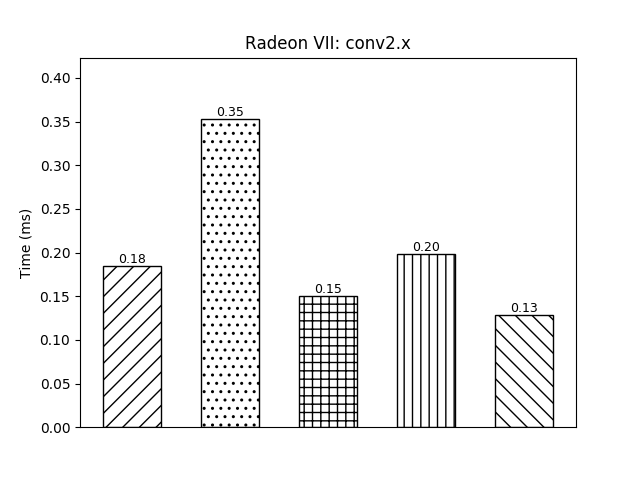
\includegraphics[width=0.24\linewidth]{Radeon_VII_conv2.png}}
\subfloat{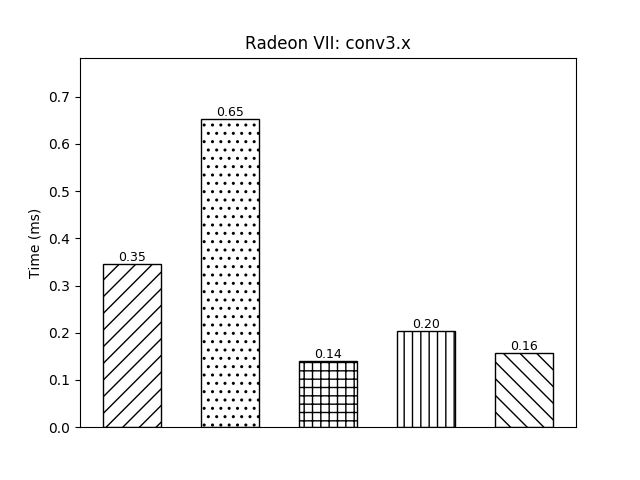
\includegraphics[width=0.24\linewidth]{Radeon_VII_conv3.png}}
\subfloat{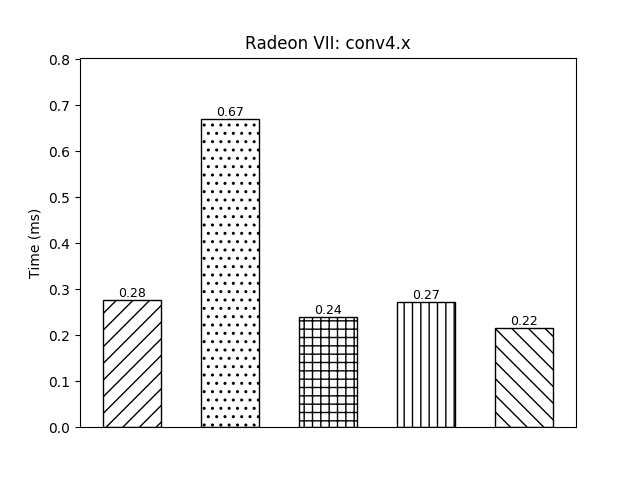
\includegraphics[width=0.24\linewidth]{Radeon_VII_conv4.png}}
\subfloat{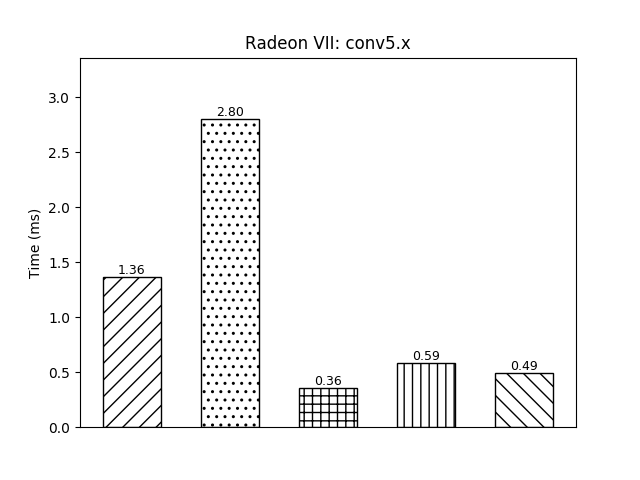
\includegraphics[width=0.24\linewidth]{Radeon_VII_conv5.png}}\\

% \addtocounter{subfigure}{-1}
\subfloat{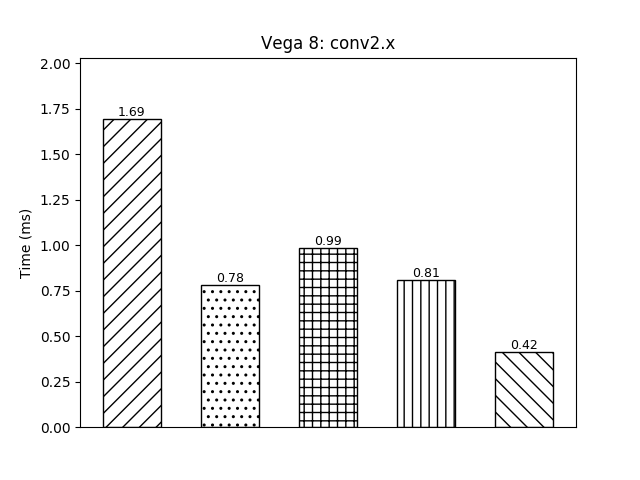
\includegraphics[width=0.24\linewidth]{Vega_8_conv2.png}}
\subfloat{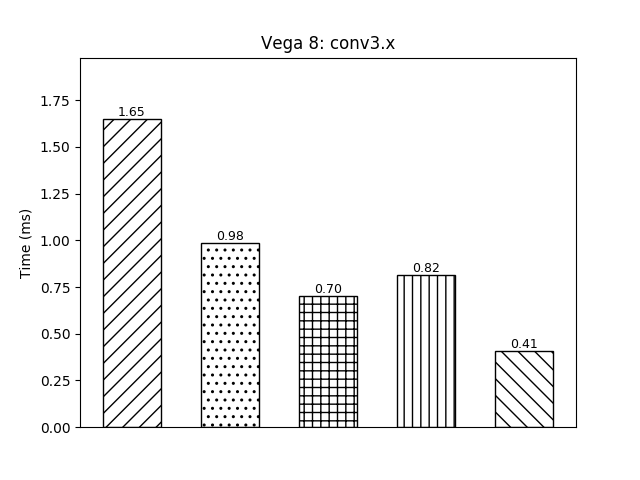
\includegraphics[width=0.24\linewidth]{Vega_8_conv3.png}}
\subfloat{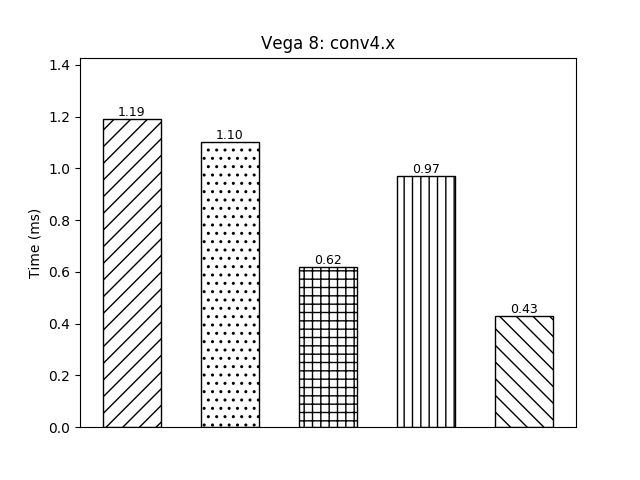
\includegraphics[width=0.24\linewidth]{Vega_8_conv4.png}}
\subfloat{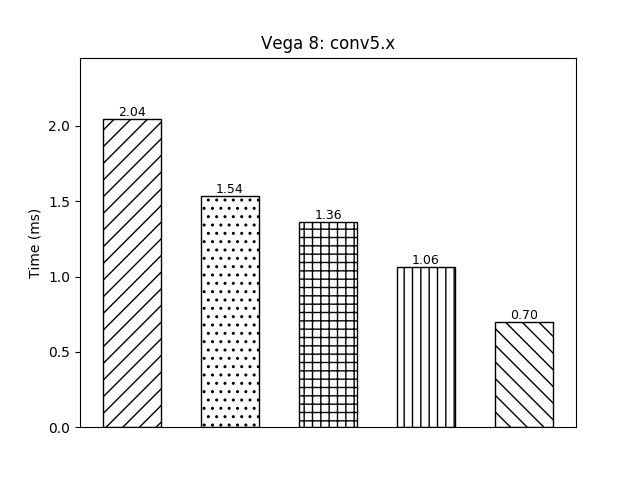
\includegraphics[width=0.24\linewidth]{Vega_8_conv5.png}}\\


\subfloat{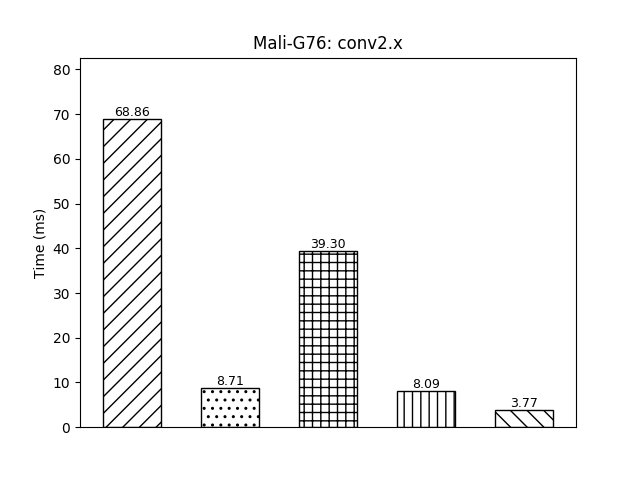
\includegraphics[width=0.24\linewidth]{Mali-G76_conv2.png}}
\subfloat{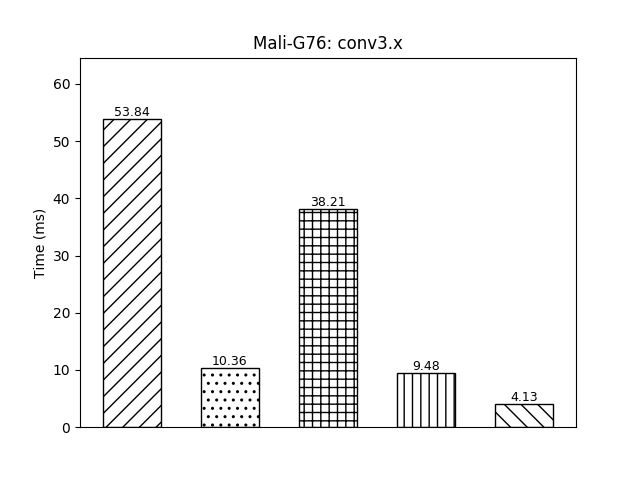
\includegraphics[width=0.24\linewidth]{Mali-G76_conv3.png}}
\subfloat{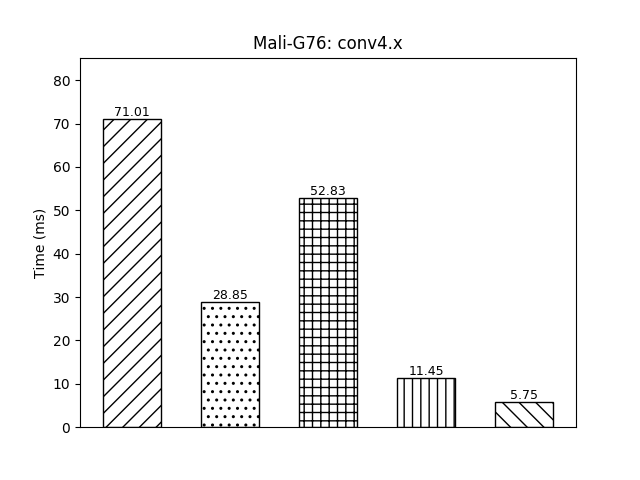
\includegraphics[width=0.24\linewidth]{Mali-G76_conv4.png}}
\subfloat{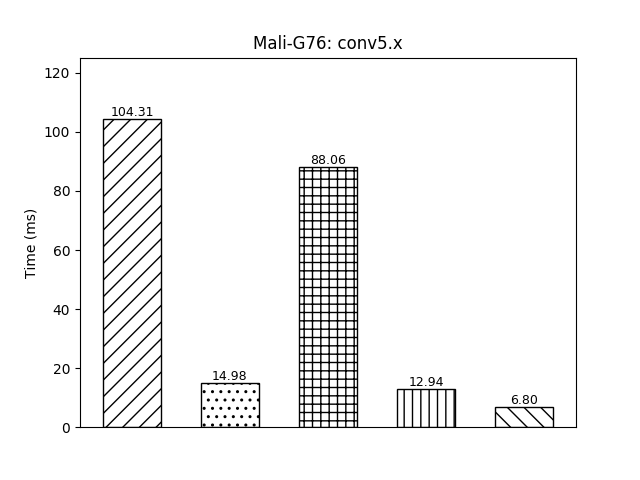
\includegraphics[width=0.24\linewidth]{Mali-G76_conv5.png}} \\


\subfloat{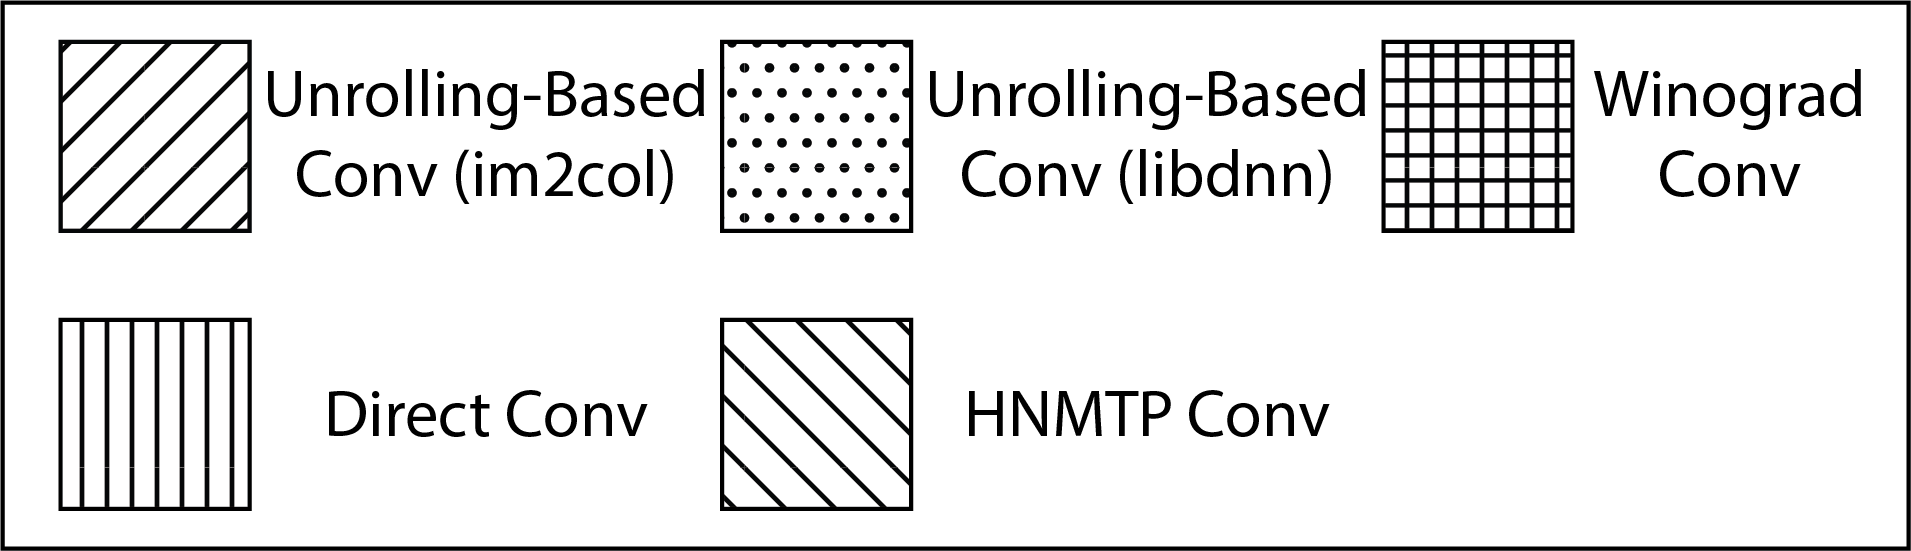
\includegraphics[width=0.3\linewidth]{legend.png}}

\caption{Comparison of the Execution Time \label{result}}

\end{figure*}


As the \texttt{libdnn} convolution algorithm eliminates the global memory access overhead of the unrolled input matrix, it overperforms the \texttt{im2col} convolution algorithm on both integrated GPUs and mobile GPUs, whose memory bandwidth is quite limited. However, on dedicated GPUs, \texttt{libdnn} convolution is more than $2 \times$ slower than \texttt{im2col} convolution, as the memory overhead is negligible with such high global memory bandwidth. It confirms our knowledge that most deep learning frameworks use \texttt{im2col} convolution algorithm for both CNNs training and testing.

The execution time of Winograd convolution algorithm is short than that of \texttt{im2col} convolution algorithm in all cases. The Winograd convolution has the fewest floating-point multiplication complexity among all algorithms. The high thread-level parallelism of Winograd convolution results in up to $3.78 \times$ speedup compared with the \texttt{im2col} convolution on dedicated GPUs, which has many compute-units. However, both the Winograd convolution and \texttt{im2col} convolution perform poorly on Mali-G72. Both of them rely on GEMM a lot, which needs large workgroup to reduce global memory access. However, as the compute-units of Mali-G72 has fewer ALUs than the other two, it favors a smaller workgroup size.

As direct convolution has too many parameters and optimization strategies, the performance varies a lot among different platforms.  On integrated GPUs, the performance of direct convolution is slightly better than the \texttt{libdnn} convolution in most cases, while direct convolution is usually slower than Winograd convolution. In contrast, the execution time of direct convolution is short than that of \texttt{libdnn} convolution on embedded GPUs. The direct convolution has around the same global memory access with \texttt{libdnn} convolution but needs less index and memory address calculations. With the saving of arithmetic operations, direct convolution overwhelms the \texttt{libdnn} on the less powerful embedded GPUs. However, direct convolution needs lots of efforts to tune the kernels to find out the optimal combination of parameters.

% Figure \ref{result} shows the execution times of convolution layers on different kinds of GPUs. It is quite surprising that the HNMTP convolution algorithm surpasses all other convolution algorithms in all convolution layers on all platforms. The thread-level parallelism is too insufficient when there is only one image, so convolution algorithms that provide higher instruction-level parallelism perform better.

% As the \textit{libdnn} convolution algorithm eliminates the global memory access overhead of the unrolled input matrix, it overperforms the \textit{im2col} one on both integrated GPUs and mobile GPUs, whose memory bandwidth is quite limited. However, on dedicated GPUs, \textit{im2col} is more than two times slower. It confirms our knowledge that most deep learning frameworks use \textit{im2col} as the GPU convolution algorithm.

% It seems quite strange that Winograd convolution performs worse on Radeno VII and Vega 8. The reason is that we serialize the group of matrix multiplications which can be combined into a single GPU kernel to take advantage of thread-level parallelism. However, it is safe to assume that the execution time ratio of Winograd convolution to \textit{im2col} convolution should be similar to that of Mali-G76. Actually, the theoretical speed of Winograd convolution (F($2\time2$, $3\times3$)) to the \textit{im2col} convolution algorithm is about $2.6 \times$, which is still slower than direct convolution, let alone the HNMTP convolution.

% In most of the experiments, the direct convolution algorithm is slightly better than the \textit{libdnn} convolution algorithm. It should be noted that the convolution filters are not cached in shared memory in our implementation. These two algorithms have around the same number of global memory accesses, but the direct convolution has higher instruction-level parallelism and less index calculation than the \textit{libdnn}. However, the direct convolution needs substantial efforts to tune the GPU kernels. It is worth to pay efforts to tune the direct convolution GPU kernels for the performance improvement, but can it be better?










In our experiments, ILP-M convolution overwhelms all existing convolution algorithms on integrated GPUs and embedded GPUs. On integrated GPUs, ILP-M convolution reduces the execution by up to $46.8\%$, compared with the second-fastest convolution algorithm, Winograd convolution. While Winograd convolution reduces arithmetic operations by additional global memory access, ILP-M convolution regards global memory access as more expensive operations. As the memory bandwidth of the GPUs without dedicated graphics memory is quite limited, even moderate global memory access may become the bottleneck. On the other hand, direct convolution is the fastest existing convolution algorithm on embedded GPUs, and our ILP-M convolution achieves $2.30 \times$ speedup with fewer efforts for GPU kernels tuning. ILP-M convolution is improved from the direct convolution algorithm and inherits all its advantages. ILP-M convolution has much higher instruction-level parallelism, as it has more independent memory instructions and arithmetic instructions to fuse and fewer register usage. 




% Of course, HNMTP convolution is much better than the direct convolution in terms of both the speed and tuning efforts. Especially on mobile GPUs and integrated GPUs, HNMTP convolution reduces the execution time by up to $50\%$ and $46.6\%$ compared with the direct convolution, respectively. On the least powerful platform, the Mali-G76 mobile GPUs, HNMTP convolution achieves speedup by $14.6 \times$ of unrolling-based convolution (\textit{im2col}), $3.1 \times$ of unrolling-based convolution (\textit{libdnn}), $10.7 \times$ of Winograd convolution and $2.1 \times$ of direct convolution. HNMTP convolution also reduces energy consumption as it has fewer global memory access. Meanwhile, tuning the HNMTP convolution GPU kernels is easier than that of the direction convolution ones, as the prior has fewer hyperparameters.


% \begin{figure*}[h!]
% \centering
% \captionsetup[subfloat]{farskip=2pt,captionskip=1pt}

% \subfloat{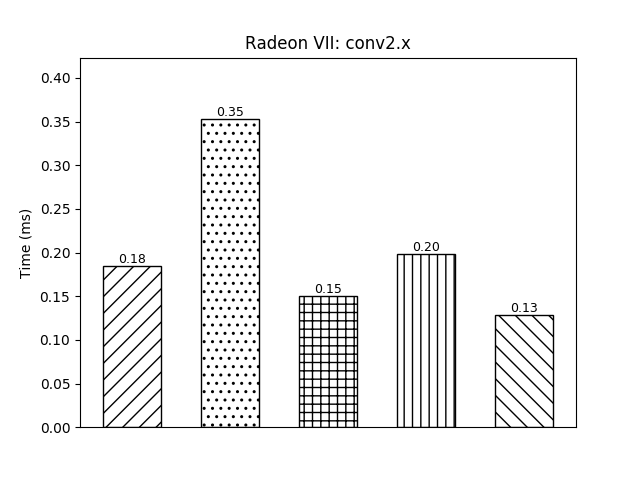
\includegraphics[width=0.33\linewidth]{Radeon_VII_conv2.png}}
% \addtocounter{subfigure}{-1}
% \subfloat[conv2.x]{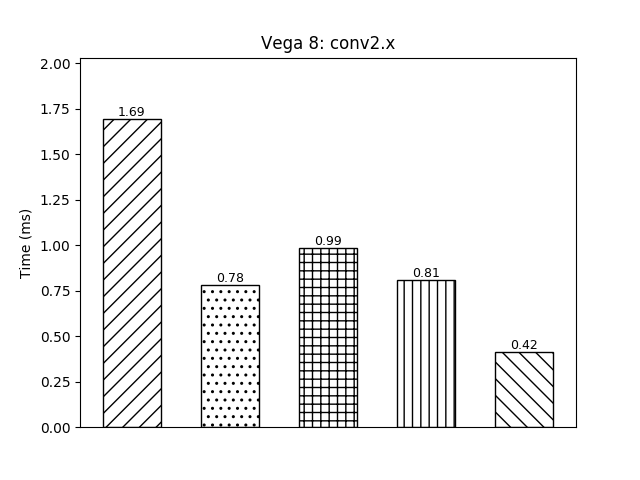
\includegraphics[width=0.33\linewidth]{Vega_8_conv2.png}}
% \subfloat{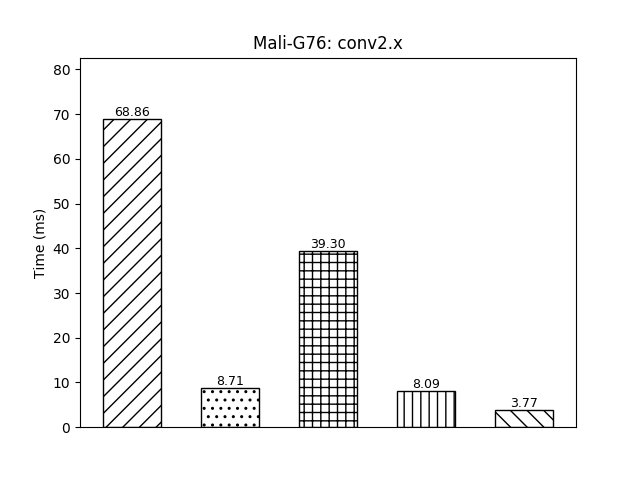
\includegraphics[width=0.33\linewidth]{Mali-G76_conv2.png}} \\

% \subfloat{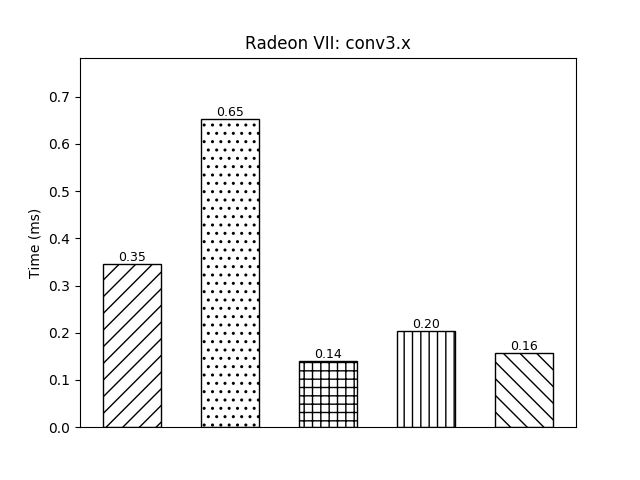
\includegraphics[width=0.33\linewidth]{Radeon_VII_conv3.png}}
% \addtocounter{subfigure}{-2}
% \subfloat[conv3.x]{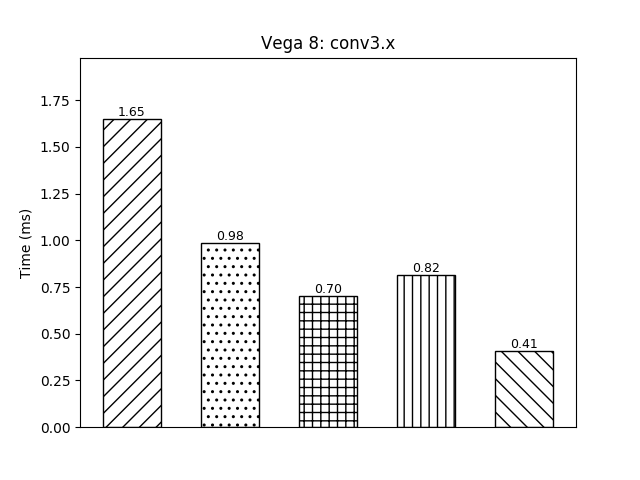
\includegraphics[width=0.33\linewidth]{Vega_8_conv3.png}}
% \subfloat{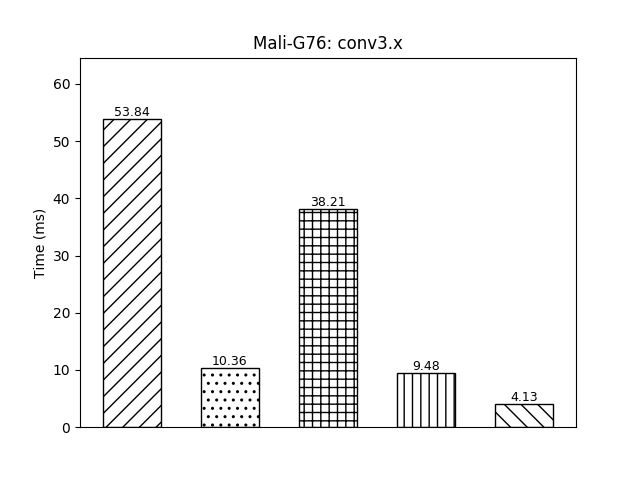
\includegraphics[width=0.33\linewidth]{Mali-G76_conv3.png}} \\

% \subfloat{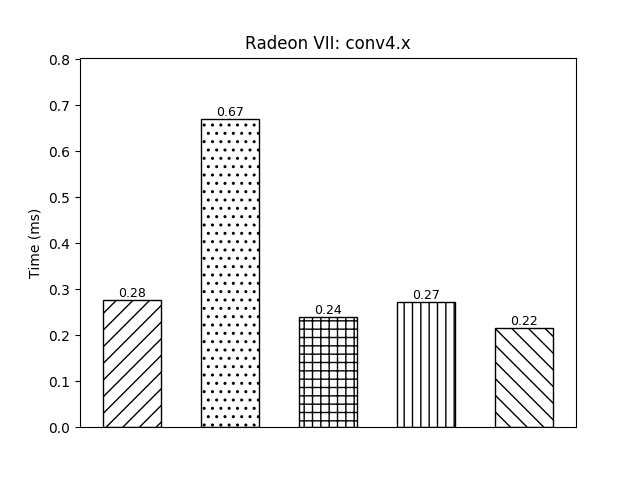
\includegraphics[width=0.33\linewidth]{Radeon_VII_conv4.png}}
% \addtocounter{subfigure}{-2}
% \subfloat[conv4.x]{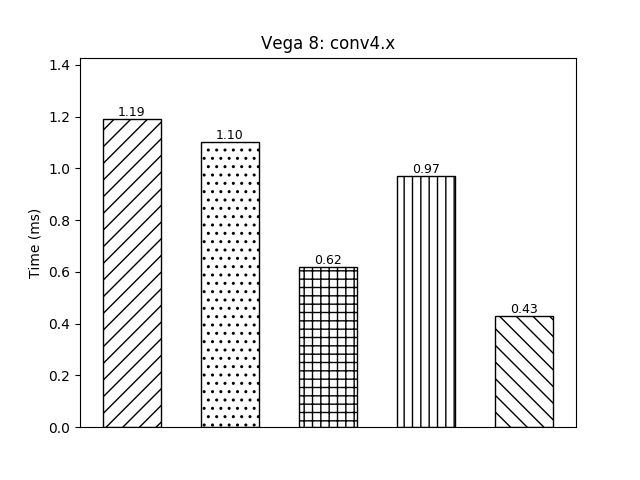
\includegraphics[width=0.33\linewidth]{Vega_8_conv4.png}}
% \subfloat{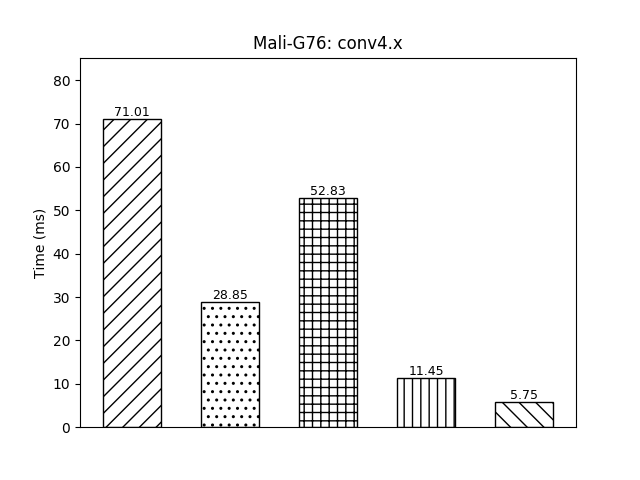
\includegraphics[width=0.33\linewidth]{Mali-G76_conv4.png}} \\

% \subfloat{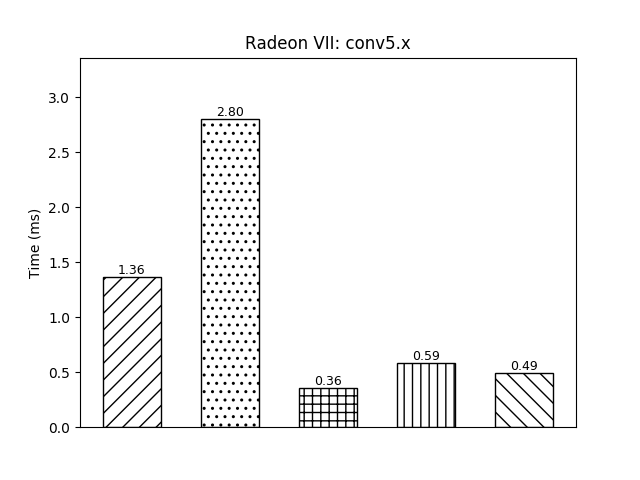
\includegraphics[width=0.33\linewidth]{Radeon_VII_conv5.png}}
% \addtocounter{subfigure}{-2}
% \subfloat[conv5.x]{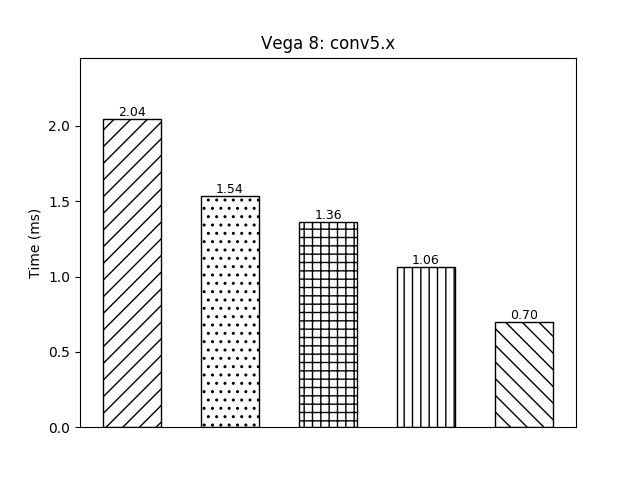
\includegraphics[width=0.33\linewidth]{Vega_8_conv5.png}}
% \subfloat{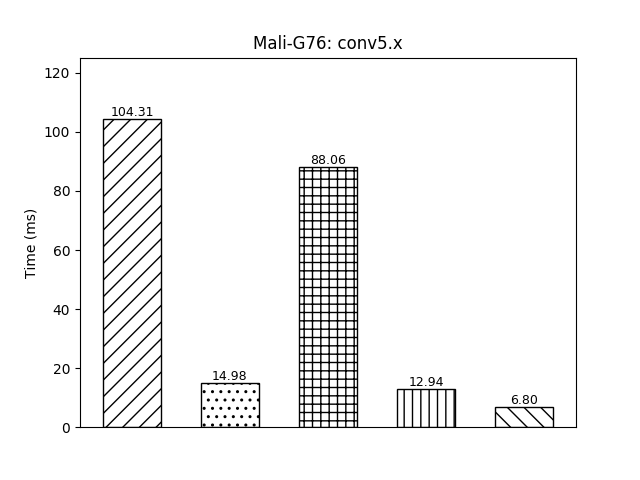
\includegraphics[width=0.33\linewidth]{Mali-G76_conv5.png}} \\

% \subfloat{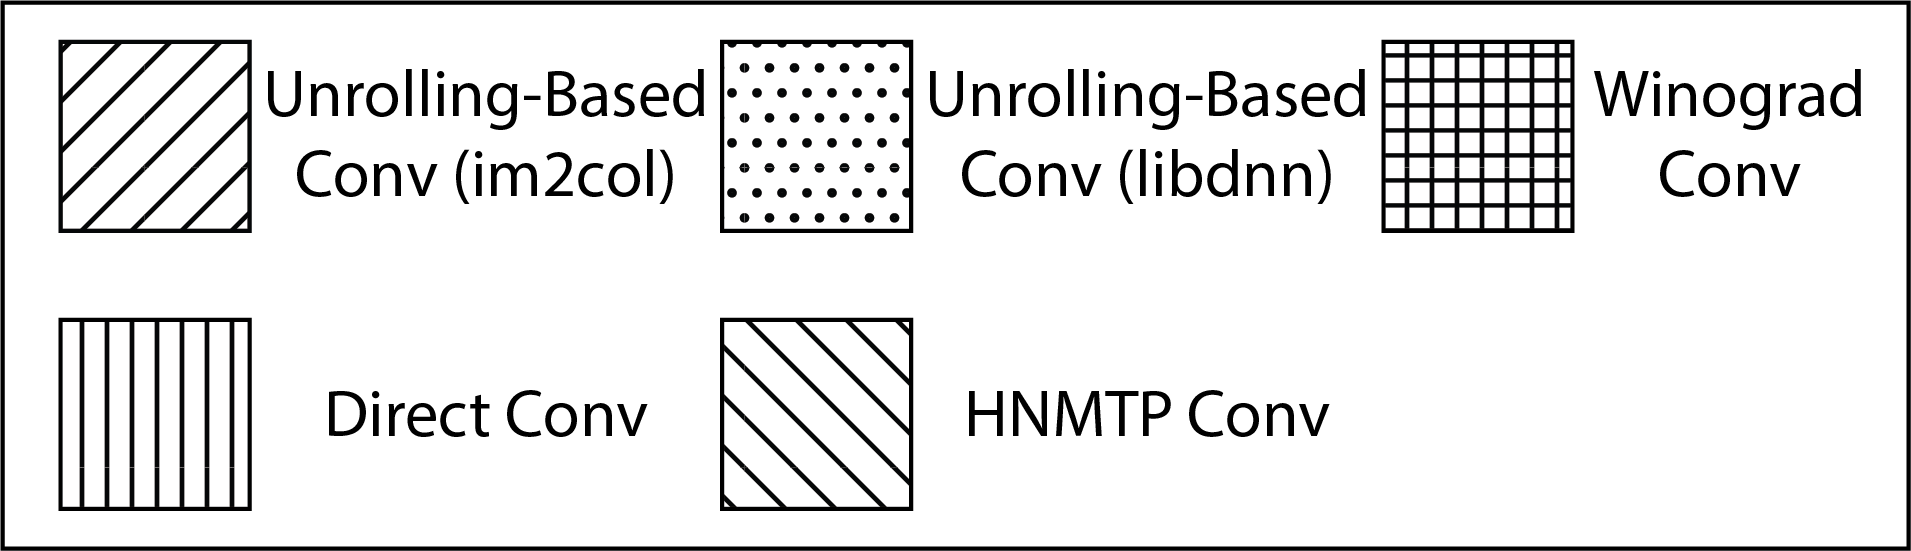
\includegraphics[width=0.5\linewidth]{legend.png}}

% \caption{\label{result}}

% \end{figure*}






\subsection{Profile}


In this section, we analyzed the performance of different convolution algorithm in the granularity of kernel-level with the profiling result in terms of memory and arithmetic instructions. We chose the most frequent \texttt{conv4.x} as the example, which has $256$ input channels and output channels and $14 \times 14$ pixels per image. We conducted the run-time profile on Vega 8 with codeXL, which provides thoughtful profiling information. The \texttt{im2col} convolution consists of the \texttt{im2col} kernel and GEMM kernel, while the Winograd convolution consists of a \texttt{trans\_from\_images} kernel, $16$ GEMM kernels, and a \texttt{trans\_to\_output} kernel. The GPU kernel that transforms the filters is ignored as the filters are constant in CNNs inference, which can be computed offline.

\subsubsection{Memory Metrics}

\begin{table*}[h!]
\scalebox{0.9}{
\begin{tabular}{l|p{2cm}|p{2cm}|p{2cm}|p{3cm}|p{2cm}}
\hline
Kernel(s)                    & Global Memory Read (MB) & Global Memory Write (MB) & Memory Unit Busy (\%) & Shared Memory Usage (Btye/Workgroup) & Shared Memory Bank Conflit (\%) \\ \hline
im2col\_im2col               & 0.20            & 1.73             & 48.91            & 0                   & 0                          \\
im2col\_gemm                 & 9.27            & 0.20             & 24.45            & 4224                & 0                          \\
libdnn\_conv                 & 2.48            & 0.20             & 15.19            & 4480                & 0.34                       \\
winograd\_trans\_from\_image & 0.20            & 0.77             & 25.01            & 1408                & 0.36                       \\
winograd\_gemm (16 times)    & 4.91            & 0.77             & 13.49            & 4224                & 0                          \\
winograd\_trans\_to\_output  & 0.77            & 0.19             & 69.96            & 0                   & 0                          \\
direct\_conv                 & 2.60            & 0.19             & 81.29            & 512                 & 4.27                      \\
ILP-M\_conv                   & 2.46            & 0.20             & 14.84            & 1024                 & 0                          \\ \hline
\end{tabular}
}
\caption{Profile Metrics Related to Memory \label{pmrm}}
\end{table*}


As shown in Table \ref{pmrm}, ILP-M convolution is one of the convolution algorithms that have the least number of global memory access. It reduces the global memory read by $74.0\%$ and $58.2\%$ and global memory write by $89.6\%$ and $88.4\%$ compared with the \texttt{im2col} convolution and Winograd convolution. With the help of L2 cache, direct convolution has similar global memory access numbers with ILP-M convolution but the memory units busy time is much higher than that of ILP-M convolution due to the duplicated convolution filters loading. 

Meanwhile, ILP-M convolution needs the least size of the shared memory per thread. Both ILP-M convolution and direct convolution cache the input images only, while other convolution algorithms also need to cache the convolution filters. However, the number of warps is usually insufficiency for single-image CNNs inference, so the usage of shared memory is usually not the bottleneck.

ILP-M convolution has no shared memory band conflicts of its main computation kernels. The threads with the same warp read the same data from the shared memory at each time. Thanks to the broadcast mechanism, only one shared memory access is needed. In contrast, \texttt{libdnn} convolution and direct convolution may need to access different data of the same shared memory bank, incurring shared memory band conflicts. The serialized shared memory accesses reduce performance and waste energy.


\subsubsection{Arithmetic Metrics}
\begin{table*}[]
\centering
\scalebox{0.9}{
\begin{tabular}{l|l|l|l|l}
\hline
Kernel(s)                    & Wavefronts & Total Vector Inst ($10^4$) & Total Scalar Inst ($10^4$) & Vector ALU Busy (\%) \\ \hline
im2col\_im2col               & 784        & 248.32                     & 343.68                     & 10.09                \\
im2col\_gemm                 & 224        & 4707.2                     & 785.76                     & 44.31                \\
libdnn\_conv                 & 64         & 6289.12                    & 1277.28                    & 45.73                \\
winograd\_trans\_from\_image & 256        & 112.16                     & 27.84                      & 10.04                \\
winograd\_gemm               & 1024       & 2469.12                    & 447.36                     & 41.24                \\
winograd\_trans\_to\_output  & 256        & 52.8                       & 2.88                       & 7.21                 \\
direct\_conv                 & 256        & 5711.52                    & 990.88                     & 31.47                \\
ILP-M\_conv                  & 32         & 3935.2                     & 43.84                      & 55.86                \\ \hline

\end{tabular}
}
\caption{Profile Metrics Related to Arithmetic \label{pmra}}
\end{table*}


ILP-M convolution uses the second least number of instructions (Table \ref{pmra}), which includes vector instructions and scalar instructions. The number of instructions issued by ILP-M convolution is only $65.4\%$ of \texttt{im2col} convolution, $52.6\%$ of \texttt{libdnn} convolution, and $59.4\%$ of the direct convolution. Even though ILP-M performs the same number of useful floating-point arithmetic, it needs less global memory address calculation and vector accesses than these convolution algorithms. As \texttt{libdnn} convolution needs to unroll the same image tile multiple times, it needs the most vector instructions due to the redundant memory address calculations.

The total number of instructions of ILP-M convolution is $1.29 \times$ of the Winograd convolution. However, there are fewer memory barriers in ILP-M convolution, which improves the instruction-level parallelism. Between two barriers, ILP-M convolution has both arithmetic instructions and memory instructions, while GEMM kernels of Winograd only have arithmetic instructions. The compilers can fuse these two kinds of instructions to hide the latency and further improves the instruction-level parallelism. As the vector ALUs are not always busy in single-image CNNs inference, high instruction-level parallelism means high vector ALUs busy time, and therefore more vector instructions can be executed in a unit time. In other words, the ILP-M convolution needs less time to execute its vector instructions, even if it has more vector instructions.

Direct convolution has the same number of memory barriers with the ILP-M convolution. However, its instruction-level parallelism is far less than ILP-M convolution. To pipeline the same number of calculations, say $N$ calculations ($N < $ \texttt{workgroup\_size}), direct convolution needs $N$ weights of convolution filters, which needs $N$ register to store as they are loaded from the global memory. In contrast, ILP-M convolution only needs one register to store one weight. With the same register usage constraints, the compiler can pipeline more calculations for ILP-M convolution.


% In this section, we analyzed the performance of different convolution algorithm with static code and runtime profile information.  We analyzed the GPU kernel code in terms of barrier number, instruction numbers between two barriers and the ratio of arithmetic instructions to memory instructions. We compared the assembly code to verify the instruction-level parallelism.





% The main difference between \texttt{im2col} convolution and \texttt{libdnn} convolution is the size of the data loaded from the global memory. The \texttt{libdnn} convolution reduces global memory loading by 73.2\%. However, as the \texttt{libdnn} convolution needs to unroll the same tile many times, its total vector instructions are 1.27 times of the \texttt{im2col} convolution.

% Compared to \texttt{im2col} convolution, Winograd convolution reduces the vector instruction by 46.8\%, including the transformation kernels. It should be noticed that the total vector instructions consist of float-point arithmetics and address offset calculation. Meanwhile, it also reduces global memory read times by 50\%. On the other hand, Winograd convolution reduces the vector instructions by 60\% and 60\% with quite a high vector ALUs utilization compared with \texttt{libdnn} convolution and direction convolution, respectively.  Even if it read more data from the global memory, the execution time of Winograd is much shorter than these two convolution algorithms.

% The size of the data loaded by direct convolution from the global memory is not that large even if every thread load the convolution filters multiple times due to the L2 cache. However, the memory unit is busy for about 81.29\%, which is significantly higher than other kernels. The high memory unit busy percentage leads to the low busy time of vector ALUs and then the poor performance. 

% ILP-M convolution overwhelms the unrolling based convolution in terms of all profile metrics. It reduces the global memory load size by 60\% and vector instructions by 20\% compared to \texttt{im2col} convolution and reduces the global memory load size by 60\% and vector instructions by 20\% compared to \texttt{libdnn} convolution. Meanwhile, ILP-M convolution has fewer barriers, leading to higher instruction-level parallelism. Therefore, ILP-M convolution has a lower memory unit busy and higher vector ALU busy.

% ILP-M convolution uses more vector instructions than Winograd convolution. However, as ILP-M has higher instruction-level parallelism, its vector ALU busy is higher than Winograd convolution by 20\%. Therefore, ILP-M convolution needs about the same time for vector instructions. As ILP-M convolution needs far less global memory access than the Winograd convolution but similar time for vector instructions, the total execution of ILP-M convolution is shorter than that of Winograd convolution.


% ILP-M convolution has about the same global memory load with the direct convolution but much less memory unit busy. In direct convolution, each filter is loaded by all threads of a workgroup, leading to high memory unit busy. In contrast, ILP-M convolution reduced the filter loading by N times, and therefore it memory unit busy is only 14.84\%. Meanwhile, as ILP-M needs less register to pipeline the memory-compute group, the instruction-level parallelism is much higher than that of direct convolution. Both the low memory unit busy and high instruction-level parallelism leads to the high vector ALUs busy. Therefore, the ILP-M convolution is faster than direct convolution.



% We chose the most frequent conv4.x as the example, which has 256 input channels and output channels and 14 images size. We conducted the runtime profile on Vega 8 with codeXL in terms of real global memory-access, shared memory usage and conflit, cache hit ratio, register usage, and ALU utilization, memory instruction numbers, register usage, and so on so forth.
 
 
% Meanwhile, we also profiled the most common convolution layer of ResNet, which has 256 input channels and output channels and each channel is a $14 \times 14$ images. The profile was conducted by codeXL on Vega 8 with Windows 10, as it is the only profiler that works. The result is shown in Table \ref{profile}. It should be noted that the sgemm of Winograd convolution is executed 16 times.











% \begin{table*}[h!]
% \caption{Profile Results \label{profile}}
% \begin{tabular}{l|l|l|l|l|l|l|l}
% \hline
% Algorithm                      & Kernel(s)  & ThreadNum & LDS  & GPRs(V+S) & VALU(\%) & GMS(R+W) & FlatVMem \\ \hline
% \multirow{2}{*}{im2col Conv}   & \texttt{im2col}     & 196*128   & 0    & 15+17     & 94.4     & 102+893  & 18       \\
%                               & sgemm      & 32*256    & 4224 & 35+25     & 92.65    & 10182+98 & 1156     \\
% \texttt{libdnn}                         & conv       & 8*256     & 4480 & 75+26     & 86.54    & 9342+98  & 2320     \\
% \multirow{3}{*}{Winograd Conv} & TransFromS & 512*64    & 1408 & 50+19     & 80.99    & 102+513  & 19       \\
%                               & sgemm (1 in 16) & 16*256    & 4224 & 35+25     & 95.73    & 1065+32  & 98       \\
%                               & TransToD   & 128*256   & 0    & 38+19     & 100      & 517+98   & 18       \\
% Direct Conv                    & conv       & 32*64     & 640  & 118+27    & 98.53    & 9627+98  & 18704    \\
% HNMTP Conv                     & conv       & 32*64     & 640  & 103+31    & 97.32    & 9331+98  & 4944     \\ \hline
% \end{tabular}
% LDS is the size of the shared memory of each workgroup in bytes, GPRs(V+S) is number of vector registers and scalar registers of each thread, VALU(\%) is the percentage of the vector ALU utilization, GMS(R+W) is the total global memory read and write in kilobytes, and FlatMem is the number of FLAT instructions of each thread.
% \end{table*}

% The the number of FLAT instructions of HNMTP convolution is much less the that of the direct convolution, as each thread of HNMTP convolution only loads its corresponding convolution filter. The usage of vector registers somehow reflects the parallelism. High vector registers usage usually indicates high ILP but low TLP, while low vector registers usage may suggest high TLP but low ILP. However, it still depends on the register usage before instruction pipeline and the number of warps. In this profile result, even both direct convolution and HNMTP convolution use about the same registers, the direct convolution has lower instruction-level parallelism due to its redundant storage of convolution filters.



\section{Conclusion and Future Work}

In this report presents the fastest convolution algorithm for single-image convolution neutral network inference on mobile GPUs. In the future, we are going to supports more tuning options, such as workload per threads and output coalescing write.





\bibliographystyle{unsrt}  
\bibliography{hnmtp_conv}  %%% Remove comment to use the external .bib file (using bibtex).
%%% and comment out the ``thebibliography'' section.


%%% Comment out this section when you \bibliography{references} is enabled.
% \begin{thebibliography}{1}

% \bibitem{kour2014real}
% George Kour and Raid Saabne.
% \newblock Real-time segmentation of on-line handwritten arabic script.
% \newblock In {\em Frontiers in Handwriting Recognition (ICFHR), 2014 14th
%   International Conference on}, pages 417--422. IEEE, 2014.

% \bibitem{kour2014fast}
% George Kour and Raid Saabne.
% \newblock Fast classification of handwritten on-line arabic characters.
% \newblock In {\em Soft Computing and Pattern Recognition (SoCPaR), 2014 6th
%   International Conference of}, pages 312--318. IEEE, 2014.

% \bibitem{hadash2018estimate}
% Guy Hadash, Einat Kermany, Boaz Carmeli, Ofer Lavi, George Kour, and Alon
%   Jacovi.
% \newblock Estimate and replace: A novel approach to integrating deep neural
%   networks with existing applications.
% \newblock {\em arXiv preprint arXiv:1804.09028}, 2018.

% \end{thebibliography}


% \appendix

% Many deep learning applications are meant for edge computing platforms, such as mobile phones, smart IoTs. One notable group of such applications is related to computer vision, whose major components are convolution neural networks. The computing of convolution neural networks is data-intensive and massively parallel, which is naturally executed on SIMD processors.

% In recent years, we have witnessed the great success of SIMD processors on mobile system-on-chip in the deep learning area, varying from GPUs to DSPs to NPUs. Even though neither Snapdragon nor Hikey reveals the architecture details of their NPUs, it is safe to assume NPUs are still SIMD processors but customized for neural networks. The NPUs should still consist of many less powerful cores that divided into several groups. Each such a group share caches and execute the same instructions. Therefore,  this report uses well-studied mobile GPUs for discussion, but the results are valid for both GPUs and NPUs.

% The main computation of convolution neural network is computation.


% Mini-batch convolution neural network training on high-end GPUs is well-studied, and many convolution algorithms are highly optimized for it. There are few study discusses single-image convolution neural network inference on mobile GPUs.

% On the other hand, the memory latency of mobile GPUs is usually about the same with GDDR6, and a single memory read needs several hundred cycles to become available.




\end{document}





% \begin{algorithm}
% \caption{Dynamic Core Allocation Algorithm \label{dcap}}
% \begin{algorithmic}[1]

% \Function{DCAM\_check\_TATD\_congestion}{ }
    
%     \State \_\_local float in\_img\_cache[TILE\_SIZE\_Y][TILE\_SIZE\_X]
%     \State \_\_private float out\_img\_cache[DIM] = {.0}



%     \For{$in\_channel \gets 1$ to input\_channels}
%         \For{$i \gets 1$ to $\lceil \frac{TILE\_SIZE}{DIM} \rceil$}
%             \State dest $\gets$ i * DIM + local\_id
%             \State destY $\gets$ dest $/$ TILE\_SIZE\_X
%             \State destX $\gets$ dest $\%$ TILE\_SIZE\_Y
%             \State srcY $\gets$ GROUP\_ID\_Y * DIM\_Y + destY - HALF\_FILTER\_SIZE
%             \State srcX $\gets$ GROUP\_ID\_X * DIM\_X + destX - HALF\_FILTER\_SIZE
%             \State in\_img\_cache[destY][destX] = input[in\_channel][srcY][srcX]
%         \EndFor
    
%         \State \Call{load image}{ }
        
        
        
%         \State \Call{barrier}{LOCAL\_MEM}
%         \For{$r \gets 1$ to filter\_dim\_r}  
%             \For{$c \gets 1$ to filter\_dim\_c}
%                 \State filter\_reg $\gets$ filter[i][local\_id][r][c]
%                 \For{$wy \gets 1$ to dim\_y}  
%                     \For{$wx \gets 1$ to dim\_x}
%                         \State output\_reg[wy][wx] += filter\_reg * in\_img\_cache[wy + r][wx + c]
%                     \EndFor
%                 \EndFor
%             \EndFor
%         \EndFor
%     \EndFor
%     \State
    
%     \For{$i \gets 1$ to dim}
%         % \State src = (get_group_id(1) * TILE_SIZE_H + (output_pos) / TILE_SIZE_W) * OUT_W + (get_group_id(0) * TILE_SIZE_W + (output_pos) % TILE_SIZE_W);
%         \State output[DIM * global\_id\_z + local\_id][i / DIM\_X][i\%DIM\_X] = out\_img\_cache[i];

%     \EndFor
    
    
%     % \For{$i \gets 1$ to dim}
%     %     \State out\_img\_trans[local\_id][i] = out\_img\_cache[i]
%     % \EndFor
%     % \State \Call{barrier}{LOCAL\_MEM}
%     % \For{$i \gets 1$ to dim}
%     %     \State output[i * output\_size + global\_id.y * output\_width + global\_id.x] = out\_img\_trans[i][local\_id]
%     % \EndFor
    
% \EndFunction


% \end{algorithmic}
% \end{algorithm}


% \subsection{Complexity of Different Algorithm}

% In this section, we discuss the complexity of different convolution algorithm in terms of barrier number, instruction-level parallelism and global memory access. 

% % Please add the following required packages to your document preamble:
% % \usepackage{multirow}
% \begin{table}[]
% \begin{tabular}{p{3cm}|p{3cm}|p{1.2cm}|p{2cm}|p{1.6cm}|p{1.6cm}}
% \hline
% Algorithm Name                          & Kernel Name         & Barrier Density & Instruction Between Barrier & Global Read & Global Write      \\ \hline
% \multirow{2}{*}{Unrolling-Based (GEMM)} & \texttt{im2col}              & N/A             & N/A                         & C * W * H   & R * S * C * W * H \\
%                                         & GEMM(M, K, N)       & K / TS          & 2 read \& 16 arithmetic     &             &                   \\
% Unrolling-Based (libdnn)                & DDR4 single-channel & 25 GB/s         & 8                           & 64          & 512               \\
% Arm Mali-G76                            & LPDDR4 dual-channel & 33.3 GB/s       & 10                          & 24          & 240               \\ \hline
% \end{tabular}
% \end{table}



% This preprint is a technical report rather than a paper. A very brief introduction to the background and problems is enough. The detailed introduction is in the appendix.

% As convolution computing is data-intensive and parallel, SIMD processors are natural choices for them. Edge computing platforms, such as mobiles phones, use GPUs or NPUs for convolution neural networks inference. As GPUs and NPUs share many common features, we use GPUs for discussion.

% There are many GPU convolution algorithms, such as unroll Conv(im2col-GEMM and libdnn), Winograd Conv, FFT Conv, and direct Conv. The im2col-GEMM and Winograd Conv are the most successful algorithms for neural network training. Both of them rely on large batch size to hide the latency, while edge computing platforms focus on executing single-batch neural network inference. Meanwhile, they do not optimize for memory. The memory bandwidth of mobile GPUs is only about 5\% of dedicated GPUs, and memory operations also cost more energy than arithmetic operation.

% In this report, we
% \begin{enumerate}
%     \item Discuss the technical difficulty of single-batch neural network inference and the bottleneck of existing convolution algorithms on mobile GPUs.
%     \item Propose a novel single-batch convolution algorithm that hides latency within each workgroup and optimizes memory operations.
%     \item Analyze the performance of our algorithm and other existing convolution algorithms theoretically and empirically.
% \end{enumerate}